\documentclass[type=bsc,colorback,accentcolor=tud8b,12pt,twoside,openright,bibliography=totoc,listof=totoc]{tudthesis}

% The following configuration file is greatly basen on a configuration file that was (as far as I know) developed by Waqas Abbas for his Master Thesis at TU-Darmstadt in 2017.
% The following configuration file is greatly basen on a configuration file that was (as far as I know) developed by Waqas Abbas for his Master Thesis at TU-Darmstadt in 2017.

\usepackage{hyperref}
\usepackage{emptypage}
\usepackage[toc,page]{appendix}
% Handling chapters & section title alignment

% no indentation for new paragraphs
%\setlength{\parindent}{0pt}

% input encoding
\usepackage[utf8]{inputenc}

% font encoding
\usepackage[T1]{fontenc}

% german or english document
% \usepackage[ngerman]{babel}
\usepackage[english]{babel}

% set line spacing to 1.5
\usepackage{setspace}
\onehalfspacing

\usepackage{listings} %code highlighter
\lstset{
	literate={ö}{{\"o}}1
	{ä}{{\"a}}1
	{ü}{{\"u}}1
}
\usepackage{color} %use color
\definecolor{mygreen}{rgb}{0,0.6,0}
\definecolor{mygray}{rgb}{0.5,0.5,0.5}
\definecolor{mymauve}{rgb}{0.58,0,0.82}

\usepackage[T1]{fontenc}
\usepackage{selinput}
\SelectInputMappings{%
	adieresis={ä},
	eacute={é},
	Lcaron={Ľ},
}

%Customize the look
\lstset{ %
	backgroundcolor=\color{white}, % choose the background color; you must add \usepackage{color} or \usepackage{xcolor}
	basicstyle=\footnotesize, % the size of the fonts that are used for the code
	breakatwhitespace=false, % sets if automatic breaks should only happen at whitespace
	breaklines=true, % sets automatic line breaking
	captionpos=b, % sets the caption-position to bottom
	commentstyle=\color{mygreen}, % comment style
	deletekeywords={...}, % if you want to delete keywords from the given language
	escapeinside={\%*}{*)}, % if you want to add LaTeX within your code
	extendedchars=true, % lets you use non-ASCII characters; for 8-bits encodings only, does not work with UTF-8
	frame=single, % adds a frame around the code
	keepspaces=true, % keeps spaces in text, useful for keeping indentation of code (possibly needs columns=flexible)
	keywordstyle=\color{blue}, % keyword style
	% language=Octave, % the language of the code
	morekeywords={*,...}, % if you want to add more keywords to the set
	numbers=left, % where to put the line-numbers; possible values are (none, left, right)
	%numbersep=5pt, % how far the line-numbers are from the code
	numberstyle=\tiny\color{mygray}, % the style that is used for the line-numbers
	xleftmargin=2.5em,
	xrightmargin=1em,
	framexleftmargin=2em,
	rulecolor=\color{black}, % if not set, the frame-color may be changed on line-breaks within not-black text (e.g. comments (green here))
	showspaces=false, % show spaces everywhere adding particular underscores; it overrides 'showstringspaces'
	showstringspaces=false, % underline spaces within strings only
	showtabs=false, % show tabs within strings adding particular underscores
	stepnumber=1, % the step between two line-numbers. If it's 1, each line will be numbered
	stringstyle=\color{mymauve}, % string literal style
	tabsize=2, % sets default tabsize to 2 spaces
	title=\lstname % show the filename of files included with \lstinputlisting; also try caption instead of title
}

%javalanguage
\definecolor{darkgray}{rgb}{.4,.4,.4}
\definecolor{purple}{rgb}{0.65, 0.12, 0.82}

%define Javascript language
\lstdefinelanguage{JavaScript}{
	keywords={typeof, new, true, false, catch, function, return, null, catch, switch, var, if, in, while, do, else, case, break},
	keywordstyle=\color{blue}\bfseries,
	ndkeywords={class, export, boolean, throw, implements, import, this},
	ndkeywordstyle=\color{darkgray}\bfseries,
	identifierstyle=\color{black},
	sensitive=false,
	comment=[l]{//},
	morecomment=[s]{/*}{*/},
	commentstyle=\color{purple}\ttfamily,
	stringstyle=\color{red}\ttfamily,
	morestring=[b]',
	morestring=[b]"
}

\lstset{
	language=JavaScript,
	extendedchars=true,
	basicstyle=\footnotesize\ttfamily,
	showstringspaces=false,
	showspaces=false,
	numbers=left,
	numberstyle=\footnotesize,
	numbersep=9pt,
	tabsize=2,
	breaklines=true,
	showtabs=false,
	captionpos=b
}


% multiple rows inside a table
\usepackage{multirow}


% consistent text for graphics
\usepackage{psfrag}

% bibliography with biblatex and biber backend
\usepackage[style=alphabetic,backend=biber]{biblatex}

% same style for URLs
\urlstyle{same}

% title not italic
\DeclareFieldFormat{title}{#1\isdot}

% colon between author and title
\renewcommand{\labelnamepunct}{\addcolon\space}

% use semicolon when multiple authors
\renewcommand{\multinamedelim}{\addsemicolon\space}

% seperate last author with semicolon
\renewcommand{\finalnamedelim}{\addsemicolon\space}

% format name
%\DeclareNameFormat{default}{\usebibmacro{name:last-first}{#1}{#4}{#5}{#7}\usebibmacro{name:andothers}}

% text for url
\DefineBibliographyStrings{ngerman}{urlseen={abgerufen am}}

% biblatex

\addbibresource{bibliography.bib}

% properly underlined url in bibliography
\usepackage{url}

% adds align command
\usepackage{amsmath}

% use graphics
\usepackage{graphicx}
\graphicspath{{gfx/}}
%\setinstitutionlogo{Images/dsp_logo.jpg}

% display pics next to each other, don't use older subfigure package
\usepackage{subfig}

% use nicer tables with footnotes
\usepackage{ctable}
\setupctable{
captionskip=0pt, framerule=0pt, nostar,
center, framesep=0pt, pos=tbp,
continued=(continued), maxwidth=0pt, super,
doinside={}, mincapwidth=0pt, table,
framebg=1 1 1, nonotespar, botcap,
framefg=0 0 0, nosideways, width=0.9\textwidth
}

% force all floats to render with \FloatBarrier
\usepackage{placeins}

% acronyms and nomenclature
\usepackage[acronym, toc, nonumberlist]{glossaries}

% links within latex


% break long URLs in toc
\usepackage{breakurl}

\usepackage{array}
\newcolumntype{L}[1]{>{\raggedright\let\newline\\\arraybackslash\hspace{0pt}}m{#1}}
\newcolumntype{C}[1]{>{\centering\let\newline\\\arraybackslash\hspace{0pt}}m{#1}}
\newcolumntype{R}[1]{>{\raggedleft\let\newline\\\arraybackslash\hspace{0pt}}m{#1}}

\setcounter{secnumdepth}{3}
\setcounter{tocdepth}{2}

% set \emph to display text italic
\DeclareTextFontCommand{\emph}{\textit}

%checkmarks for table
%\usepackage{amssymb}% http://ctan.org/pkg/amssymb
\usepackage{pifont}% http://ctan.org/pkg/pifont
\newcommand{\myes}{\ding{51}}%
\newcommand{\mno}{\ding{55}}%
\renewcommand{\emph}{\textit}%



 %TODO: make \emph display italic
\begin{document}
	
	\pagenumbering{roman}
	% Title page

% #1: English title
% #2: German title
% fromat: \thesistitle{english title}{german title}
\thesistitle{A Debugging Tool for Javascript Reactive Libraries}{}
% Name of Author
\author{Waqas Abbas}

% Dept name
% logo of included for thesis thesis

\department{Fachbereich Informatik}

% Group name. {leave it empty}
\group{Reactive Programming Technology}

% In date
% \date{21.03.2011}
\date{05.06.2017}

% #1: Name of Professor
% format: referee{prof 1}{prof 2}{prof 3}
% leave other twoo options empty
\referee{Prof. Dr. Guido Salvaneschi}{M.Sc. Pascal Weisenburger}{}
		\makethesistitle
		
		\chapter*{Ehrenw\"ortliche Erkl\"arung}
	Hiermit versichere ich, die vorliegende Bachelorarbeit ohne Hilfe Dritter und nur mit den angegebenen Quellen
    und Hilfsmitteln angefertigt zu haben. Alle Stellen, die aus den Quellen entnommen wurden, sind als solche
    kenntlich gemacht worden. Diese Arbeit hat in dieser oder \"ahnlicher Form noch keiner Pr\"ufungsbeh\"orde vorgelegen.
    Die schriftliche Fassung stimmt mit der elektronischen Fassung \"uberein.
	\vspace{1.5cm}
	
	\noindent Darmstadt, den 02. Januar 2018\hfill Benedikt Gross
%	\chapter*{Declaration of Authorship}

I herewith formally declare that I have written the submitted thesis independently. I did not use any outside support except for the quoted literature and other sources mentions in the paper. I clearly marked and separately listed all of the literature and all of the other resources which i employed when producing this academic work, either literally or in content. This thesis has not been handed in or published before in the similar form. Written version of this thesis corresponds to the electronic version.

\vspace*{3cm}
\noindent
\begin{tabular}{c} Darmstadt, 05 June 2017\\\rule{5cm}{1pt} \\ (Place, Date)\end{tabular}  \hfill \begin{tabular}{c} \\ \\ \rule{5cm}{1pt} \\ (Waqas Abbas)\end{tabular}
	\cleardoublepage
	
	\begin{abstract}
			Abstract
	\end{abstract}
	
	\cleardoublepage
	\tableofcontents
	%\listoffigures
	%\listofcodes
	%\lstlistoflistings
	%\listoftables


	\pagenumbering{arabic}
	\chapter{Introduction} \label{ch:Introduction}
Introduction Header Placeholder

\section{Background}
% Reactive Inspector and previous CRI mentioned

\section{Motivation}
% increase usablity of CRI
% advance to eventually be used in production environment


\section{Our Contribution}

In the last two sections, we introduced reactive systems, ...


As a summary, this thesis makes the following contributions:

\begin{itemize}

	\item Item 1
	\item Item 2
	

\end{itemize}


\section{Outline}

Outline Placeholder

	\cleardoublepage
	\chapter{State of the Art} \label{chap:State of the Art}
% introduction

\section{Implementation of Reactive Systems}
	\subsection{Reactive Programming}
	%"Reactive programming provides dedicated language abstractions for reactive software. Reactive programming relieves developers from manually updating outputs when the inputs of a computation change, it overcomes a number of well-know issues of the Observer design pattern, and it makes programs more comprehensible." [github, rxScala guido] Its also declarative instead of imperative.
	% reactive programming is in general not asynchroneous but it can be used in async context.? (waqas says something different for RXjs)
	% observables, difference to Observer design pattern:
		% observables in a reactive system return/provide multiple values (a stream) instead of just the current state.
		% "Observables provide abstractions over a stream of events. Promises are synchronous executables with a single return value, whereas observables are asynchronous executables that return multiple values over time." [pradeep]
		%"The data produced by the producer is stored in observable which the consumer consumes."[Pradeep]
	% observables are also called signals[wikipedia] = values that vary over continuous time -> or in RxJs Observables, Bacon Properties
	% events = events which have occurrences at discrete points in time -> RxJs Subject, Bacon EventStream
	% "observables" are functions that tie an observer to a producer. A producer creates values over time. An observer reacts to the values of a producer and notifies all subscribers (in a push based system).
	%operators: "Each operator outputs an another observable without modifying the original data streams." [Pradeep]
	% push and pull based: 
		%"Push-based systems take events and push them through a signal network to achieve a result. Pull-based systems wait until the result is demanded, and work backwards through the network to retrieve the value demanded." https://en.wikipedia.org/wiki/Functional_reactive_programming
	% cold and hot observables https://medium.com/@benlesh/hot-vs-cold-observables-f8094ed53339
			% -> author: "RxJS 5+ Lead, Software Engineer at Google, RxWorkshop.com. Own view, not the companies"
		% cold: the subscribe call creates the producer - one producer (e.g. a websocket raising events) is created for each call to subscribe, it gets destroied if the observer unsubscribes -> unicast
		% hot: all calls to subscribe (usally) share one producer - multicast
		% Rx Subjects - functions as both observer and observable, multicast but will terminate if the last subscriber is unsubscribed, can not be reused after termination or if in error state. "It multicasts. All observers passed to it via `subscribe()` are added to an internal observers list."
			% "Armed with our Rx Subject above, we can use a bit of functional programming to make any “cold” observable “hot”:
			%function makeHot(cold) {const subject = new Subject();cold.subscribe(subject); return new Observable((observer) => subject.subscribe(observer));}
			%Our new `makeHot` method will take any cold observable and make it hot by creating a subject that is shared by the resulting observable."
			% in RxJs that is e.g. publish or share
	
	\subsection{RxJs and BaconJs}
	% Though there are other Javascript implementations of the reactive design pattern like https://github.com/stoeffel/awesome-frp-js,
	% kefir, cyclejs
	% this thesis focuses on RxJs and BaconJs, because these are the one the extension currently supports.
	
	%RXjs
	%var button = document.querySelector('button');
	%Rx.Observable.fromEvent(button, 'click')
	%.throttleTime(1000)
	%.scan(count => count + 1, 0)
	%.subscribe(count => console.log(`Clicked ${count} times`));
	% The essential concepts in RxJS which solve async event management are:
	%Observable: represents the idea of an invokable collection of future values or events.
	%Observer: is a collection of callbacks that knows how to listen to values delivered by the Observable.
	%Subscription: represents the execution of an Observable, is primarily useful for cancelling the execution.
	%Operators: are pure functions that enable a functional programming style of dealing with collections with operations like map, filter, concat, flatMap, etc.
	%Subject: is the equivalent to an EventEmitter, and the only way of multicasting a value or event to multiple Observers.
	%Schedulers: are centralized dispatchers to control concurrency, allowing us to coordinate when computation happens on e.g. setTimeout or requestAnimationFrame or others.
	%"The subscribers are not locked in a synchronous request and there can be an infinite sequence of next emissions from the observables to the observer." [Pradeep] although subscribing is in general a synchroneous operation.
	%"completed and error functions	being defined at the observer, which are invoked by the observable on respective events. This lets the observer know that an observable has exhausted sending values, or an error has occurred	when performing an operation on the observable." [Pradeep]
	%"Subjects can be both observable and an observer[37]. It is a special type of observable which	allows values to be multicasted to many observers" [Pradeep]
	%"Unsubscribing is an optional feature in RxJS as RxJS handles this by default but it makes sense to unsubscribe manually by a user if the source observable is emitting the values continuously and the user does not need values after a specific point of time." [Pradeep]
	%"With the support of RxJS, we can convert multiple values, arrays, events into observables."[Pradeep]
	% - current version in development 6.0.0-alpha.2, stable: 5.5.6
	% - github stats 31.1.2018 18:22 for current active version (they changed repositories multiple times): watch: 387 star: 10,540 fork: 991 contributors: 185 but since they changed the repository the total numbers for all versions are much higher.
	% licence: Apache 2.0 latest commit: 30.01.2018
	% first release on github: version 2.2.0 01.03.2013
	
	%Baconjs: 
	%Generally, this is how you implement an app with Bacon.js. Capture input into EventStreams and Properties - Transform and compose signals into ones that describe your domain. - Assign side-effects to signals.
	%EventStreams (distinct events) and Properties (values that change over time). 
	%$("#username input").asEventStream("keyup").map(function(event) { return $(event.target).val() }).toProperty("")
	% "In Bacon, these are two flavors of Observables. EventStreams and Property are two basic concepts	of Bacon.js that are basically known as events and behaviours in the literature of FRP." [waqas]
	% - BaconJS does not have cold observables [ref baconjs github - For RxJs Users]
	% - "Error handling is also a bit different: the Error event does not terminate a stream. So, a stream may contain multiple errors. To me, this makes more sense than always terminating the stream on error; this way the application developer has more direct control over error handling. You can always use stream.endOnError() to get a stream that ends on error!" [baconjs github]
	% - it has the "spy" feature which greatly reduces the required effort to create complementary tooling like CRI or RxFiddle. It can also be used to easily create extensive logging.
	% - created because "Bacon.js exists largely because I got frustrated with RxJs, which is a good library, but at that time didn't have very good documentation and wasn't open-source. Things have improved a lot in the Rx world since that. Yet, there are still compelling reasons to use Bacon.js instead. Like, for instance, more consistent stream/property behavior and (arguably) simplicity of use." [baconjs github]
	% - current version 2.0.0
	% - github stats 31.1.2018 18:22: watch: 156 star: 5,839 fork: 328 contributors: 83
	% licence: MIT latest commit: 30.01.2018
	% -> has a smaller community than RxJs
	% first release on github: version 0.7.90 08.03.2017
	

	\subsection{Debugging Reactive Code}
	% due to reactive programming being declarative ... [github, guido rxScala]
	% short-comings of standard debuggers with reactive systems:
		% - stepping through reactive libarary code to track down bugs
		% - unconditional breakpoints in lambda functions will trigger to often to be useful 
		% - non-linear code execution makes step by step debugging hard -> "step over" is rarely useful and "step into" needs to be used multiple times for chained functions to iterate to the desired part, because "step over" will skip the whole line [verify with VS, IntelliJ, Webstorm, Chrome debugger].
		%- "lack of abstractions" and "mismatch in the mental model" [paper guido1]
		% - "Missing dependencies are hard to detect with traditional debuggers." [paper guido1 4.1]
	% - unit tests and do-debugging for Rx: https://msdn.microsoft.com/en-us/library/hh242967(v=vs.103).aspx to reduce the effort of adding do-statements each time a bug is tracked down, the developer can add logging functionality and use that in the do statement. https://shiny.rstudio.com/articles/debugging.html #"The Reactive log" where a visualization is later used on the log to create a simple dependency graph containing code pieces as nodes.
	% other systems that do
	% - Reactive Inspector for scala https://guidosalva.github.io/reactive-inspector/ is an extension of Scala IDE for Eclipse. Reactive Inspector is a project started and maintained by Guido Salvaneschi at the Software Technology Group - Technical University of Darmstadt, Germany and many people have contributed.
		% - Many features and the basic concepts that are implemented in CRI originate from RxScala Reactive Inspector. Dependency graph in the so called Reactive Tree, Tree History, History Queries, Reactive Breakpoints, Node search/dependencies/dependents. They are described in details in [Chapter: Previous CRI]
		% -"Tree Outline: Tree Outline In a large dependency graph it is sometimes hard to navigate the reactive tree. This view shows you at a glance where you are in the graph and helps you jump quickly to a different area of the graph."
	% - reference to rxfiddle in later section

\section{Previous and Related Work}
	\subsection{The Chrome Reactive Inspector}
		\subsubsection{Master Thesis by Waqas Abbas}
		% main focus of the thesis
			% - proof of concept
			% - how to intercept calls to reactive framework
			% - how to retrieve additional details for each node like the variable name via instrumentation of the source code to give context to observables shown in the dependency graph
		% implemented result of the thesis in short
			% - reactive breakpoints
			% - history queries
			% - Bacon support and partly support for Rx
			% - dependency graph, nodes, edges, zoom, highlighting of current node
			% - instrumentation, dynamically reloading of the page to intercept the javascripts for instrumentation
			% - first batch of test applications
			% -> focus on new implementation and prototypes of features and less on maintainability and reliability.
			% -> proof of concept
		
		\subsubsection{Master Thesis by Pradeep Baradur}
		% main focus of the thesis:
			% support for all RxJS operations and RxJS Subjects -> hard to implement, because there is no uniform way like the Bacon.spy method. For details on the general approach see [ref to pradeep thesis]. For source code see "rx-interception.js"
		% new features introduced:
			% - support for all operations and Subjects in RxJs
			% - loading of some CRI content scripts only when the CRI panel is opened. Istrumentation only when CRI panel is opened.
			% - find dependencys, dependents
			% - added many test applications
			% - improved reliability
			% - less focus on maintainability but move the project further to being usable in a production environment by adding framework feature support.
			% - rearranged UI, changed many styles to defaullt jquery-ui layout.
		
		\subsubsection{Merging previous efforts}
		%- took chrome-reactive-inspector 2 as base and merge all later developed features into it, piece by piece. manually copied changes by Pradeep from Waqas's repository. Hard to detect, changed to match other variable names before committing.
		% - uncompatible git histories - solvable but not much use since the files had separated so much in text character changes, though not so much in logic -> renames and splitting of files
		% - access to many global variables made tracking down dependencies of components hard with mixed contexts - some files with the window object corresponding to contentscripts in the same directory as files with a window object corresponding to the extensions window.
		%TODO: change tone to always present problems as general difficulties instead of shortcomings
		% - merged additional features of Abbas with framework support from Pradeep
		
		\subsubsection{"Special Curicumstances"}
		% demo version of jalangi
		% instrumenting files via scanning the html for script tags
		% -> will not work for module loaders like require.js or ecma6
		% -> will not work with bundled javascript code - but since in development there should be a non bundled version available not 
		% a big problem in javascript. But for Typescript since the extension does not support it and when compiling there may already be bundling in place. (#add some text from future here#)
		
		% Shared context through "new Function" that breaks the separation enforced by chrome. To increase consistency and prevent different execution contexts the previous eval was replaced with "new Function" but this does not reduce the security risk.There are other options to execute scripts from a chrome extension but since some of the extension scripts need to share the Rx or Bacon object with the inspected pages javascript files there is no other way. ofcorse that breaks the normal isloated world and intodruces a new set of problems like conflicting names. The security risk involved in executing a foreign script in a "trusted" extension context could be reduced if a sandbox was used as described in https://developer.chrome.com/extensions/sandboxingEval. Then all the inspected pages content scripts and some special recording scripts could be executed in that sandbox and transmitt the recorded nodes back via message passing.
		% - Dangers of using eval -> execution in current context. if called from other function, "this" might change. Function() for global with window passed to execute in original context.
		%- Note that  files that are not selected for instrumentation will still generate nodes in the graph, because the Rx and Bacon frameworks will still record interactions, just the information provided by instrumentation is missing.
		%- The Bacon and Rx scripts are prevented from loading so the extensions own files can be used. This is accomplished by filtering all referenced js files in the inspected page for any Bacon or Rx library files and excluding them from the loading process. They need to match version exactly though. This is necessary to guarantee that both work with the same Rx/Bacon object.
	

	\subsection{RxFiddle}
	% RxFiddle is the main competitor with CRI since it is the only other tool (that we are aware of) that tackels debugging for reactive javascript systems. Currently the only reactive framework that is supported is RxJs.
	% features of RxFiddle
	% limitations: 'one of the limitations of RxFiddle is ... which we tackeld in this work.
		% - requires more setup to use with web sites that have DOM logic and applications with more than one Javascript files, although it is possible according to the author [ref rxfiddle attached].
		% - the variable names in the source code are not displayed in the ui. RxFiddle instruments RxJs to collect its data, not the source code itself like CRI.
		% - fast updating observables like "interval" since each value update creates a new marble for the observable, the view becomes encoumbered fast with this type of observables. As of this moment CRI also generates one or more steps for each update (if the node is not explicitly excluded), but it is easier to examine the value of a node in the first or last few steps (jump to the step and use the next/previous button). CRI can also query the result which provide means to cope with large dependency graphs or histories. In RxFiddle the limitating factor for the fine grained stepping is the available space and resulting overplotting of the value-marbles since the examination is implemented via tooltips on mouseover. For performance comparison see [Evalutation chapter section Performance Improvements].
		% - like the author explained in "https://github.com/hermanbanken/RxFiddle/issues/6" the web app can not work with large applications properly. The displaying of large applications in one graph is hard for both tools [reference to Contributions chapters], but RxFiddle needs more spaces for a single reactive operator than CRI. A large dependency graph with descriptive nodes is easier to examine than a large marble diagram that only shows information on nodes in tooltips except in the details view of a currently selected node so finding the desired node/operation is not as easy. RxFiddle also has performacne issue while rendering huge diagrams according to the author. RxFiddle would porbably need another view to appropiately cope with such large applications to help the user navigate and give an overview, although for mid-sized applications the graph on the left side where a user can choose which operation to examine can serve this purpose - As mentioned earlier RxFiddle does not porvide variable names which may lead to confusion of nodes if similar observables are in the same application.
		% As of now, CRI does not support multiple variables having the same name. The author describes some other options like priority ranking in the issue [ref].
		% - as mentioned erlier RxFiddle onyl supports RxJs while CRI also supports Bacon.js
	% - The author plans to support multiple collectors in the future for web applications, RxScala, RxJava, RxSwift and/or RxNet (source: "https://rxfiddle.net/tutorials.html#attached") which would provide the necessary data collection on one of these platforms and transmit this data to the RxFiddle tool/web-application to be able to use the same debugging environment (RxFiddle) with any of these platforms.



% end of state of the art chapter
%----------------------------------------------------------------------------
%latex sample code:



\begin{figure}[!h]
	\centering
	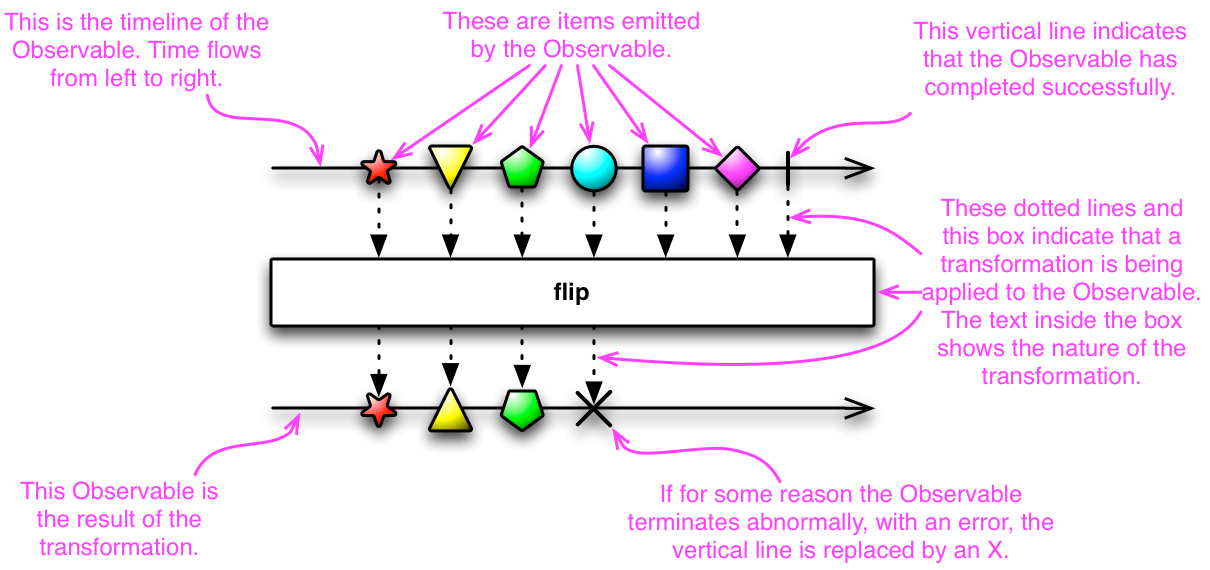
\includegraphics[scale=0.5,trim=0 0 0 0]{gfx/rxjs-reactive-pattern2.png}
	\caption{Reactive pattern \protect\cite{ReactiveXobservable}}
	\label{fig:rxjs-reactive-pattern}
\end{figure}

\textbf{Observable and Observer}\\
Placeholder

\textbf{Operators}
\label{subsec:Operators}\\

\textbf{RxJS Code Structure}\\
Placeholder
\begin{lstlisting}[language=JavaScript, caption=RxJS Simple Example, label={lst:RxJS_Simple_Example}]
// 1. Srouce Observable Creation
var sourceObservable = Rx.Observable.interval(1000);
// 2. Transformation by applying different operators
var transformedObservable = sourceObservable.map(function(x) {
		return x * 10;
	})
	.filter(function(x) {
		return x !== 20
	})
// OUTPUT
Next: 0
Next: 10
Next: 30
Next: 40
Next: 50
Completed
\end{lstlisting}

\subsection{Bacon.js}

\textbf{EventStream and Property}\\
Placeholder


	\cleardoublepage
	\chapter{Contribution}
\label{ch:Contribution}
In this chapter, we discuss the features and changes introduced in this thesis as well as other implementation options and why we chose our approach over the others.
In the following sections "Observable" is used to denote an actual RxJS Observable and also as a placeholder for any Reactive entity from RxJS or BaconJS in lack of a better term.

\section{Advancing the User Interface}
The User Interface (UI) is an important part of every application. A good UI helps the user focus on the task at hand by displaying the necessary information required for that task. For a website this task may simply be to find gather information about the subject of the website itself. An IDE usually provides many tools the user can use and reduce the manual work of the user by automating some steps of the development process. There are many factors that need to be taken into account when developing a new UI or changing an existing one. A UI should normally be designed to match the special use-cases the application was designed for while also keeping some familiar elements to guide the user. The main reason to keep a somewhat familiar look or have a certain part of the UI match what the user expects and knows from other applications in his domain is that the user already knows how to interact with familiar elements and does not have to learn how to use them from scratch. It is also important to consider some of the characteristics of human cognition. To explain them all in detail is beyond the scope of this thesis. To solve this type of problems if a main target of the Interactive Graphics Systems Group (GRIS) at TU-Darmstadt and many other groups worldwide are working in this field. In the following paragraph we examine the changes to the UI of CRI we implemented in this thesis and the reasoning behind these changes.
  
\textbf{Reducing the cognitive load on the user}
The main goal of the changes to the UI we implemented in this thesis is to reduce the cognitive load on the user. If the user has to concentrate and search for information they need to achieve their task and not having them presented in an easy to find and understand manner, half of his attention is already occupied. It cannot be used to work on the task and achieve their actual goal.

The first change we introduced to reduce the cognitive load on the user is to move some input elements to a menu that is displayed at the top of the CRI's UI. Nearly every desktop application and many websites (e.g. http://reactivex.io/rxjs/, Windows File Explorer, Eclipse, Microsoft Paint, Adobe PDF Reader and many more) use a menu at the top of the UI. This adds structure and also removes many buttons from the normal working space which can then be used to display more relevant information. The user knows that the buttons are in the menu and searches though it on demand. The buttons hidden in the menu bar do not require space or attention by the user at other times, except for the space required by the menu itself. We examined our own usage frequency, how often we use a certain input element, and estimated the tasks that include the input element to determine which elements should be part of the main UI and which should be hidden in a menu (or closeable panel for inputs other than buttons). We found that we rarely used the \emph{Reset}, \emph{Download} and \emph{Pause/Resume} buttons. The latter was used most among them and since CRI does not actually have loads of buttons yet, we decided to place it directly in the menu bar instead of moving it into the submenu used for the other rarely used buttons. The \emph{Pause/Resume} button is also the only one of those buttons used in a normal workflow, i.e. in the special case of working with Rapidly updated Observables (see section \ref{sec:RapidlyUpdatedObservables}) it is used regularly to counter performance issues or focus on a specific part of the execution.
The other buttons of the UI are part of a specific feature of CRI and cannot be moved away from other elements that belong to the features. These features from left top to bottom right are the Instrumented Files list, History Queries, and the navigation through the results, Reactive Breakpoints, Search, History Navigation and the Dependency Graph. The Dependency Graph and History Navigation are closely tied together and represent the main part of CRI. They are the working area where the focus of the UI should be. The other features are complementary to them support the user ins examining their content. Although CRI can be used effectively without History Queries and Reactive Breakpoints they can help the user in almost any task. Reactive Breakpoints may even be mandatory to discover some issues with an application that otherwise could not be detected without a much greater effort (similar to normal Breakpoints in traditional IDEs). While the Dependency Graph with its History is just another way to provide an abstract representation of Observables and Dependencies then the Marble Diagrams used in RxFiddle, Reactive Breakpoints are currently exclusive to CRI. In conclusion, History Queries and Reactive Breakpoints should be a permanent part of the UI, therefore, we decided to keep them where they were positioned in CRI2 - above the History Navigation. The Search feature is not as important in most tasks. The highlighting of a specific node, its Dependencies or Dependents is only useful for applications with large Dependency Graphs. Small graphs can easily be searched for the required information manually with one look. Therefore, the Search feature could be moved to a closeable panel that is only opened on demand. The search implemented in most IDEs opens when the user presses CTRL F or clicks the search button in the menu. The reason we did not move the feature to a closeable panel yet is simply that the area of the UI where the History Query and Reactive Breakpoints input elements are placed provides enough space (with standard screen resolutions sizes for desktop computers) to keep the Search there as well. With the current UI, the space is otherwise left empty. %TODO: sentence correct? after fixing close paragraph again
 However, as soon as these parts of the UI change or another feature is introduced, the Search should be moved to a closeable panel. The remaining feature is the Instrumented Files list. It is used as a scoping feature to select which files should be instrumented. For small to medium-sized applications the list of files will normally include all relevant JS files and will not be changed at all. It is, therefore, reasonable to move it from the main UI to free the space that could then be used to increase the size of the Dependency Graph canvas. After examining the outcome of this change we found, however, that in case the user switches to another application that requires other files to be instrumented or forgot to include a JS file in the list, it can be really difficult to detect the reason why the Dependency Graph is not showing the expected result. If the Instrument Files list is moved from the main UI, the user may lose track of the fact that not all JS files are automatically instrumented or, if they decided to instrument only a subset of JS files as a filtering measure, that the >filter< is still in place. It is also easier for new users to comprehend the need to select files for instrumentation if the list is part of the main UI. This could be mitigated by adding a dialog informing the user at the first start of CRI, but for this reason, in addition to the reasons mentioned above, we decided the benefits outweigh the downside of a small part of the UI being occupied by a rarely changed input. Therefore, we kept the Instrument Files list at the top of the UI and also added a red border around the text input as a validation error in case the list is empty to help make new users aware of the missing input.

To further decrease the cognitive load when working with CRI, we removed any text from nodes and their tooltips that do not carry any value. The less text is displayed in the UI, the less a user has to read to find the information that they require.%TODO: sentence correct? after fixing close paragraph again
 This is most significant for the \emph{Method} field in the tooltips since most Observables do not correspond to a method and the field, therefore, is empty for most nodes. The \emph{Value} field is usually set, but if there is no value, there is no need to keep the label for the field. The same information is available to the user if the label for \emph{Value} is simply omitted in that case.
It is, however, important to display values that explicitly denote an \emph{empty} value like \emph{undefined}, \emph{null}, or -1 (for a value that carries positive numbers if it is set). The \emph{Name} field is also not set for every node. Figure \ref{fig:Nodes} shows an example of nodes from CRI2 with all field as well as nodes from the current version.

\begin{figure}[!h]
	\centering
	\subfloat[CRI version 2.0]{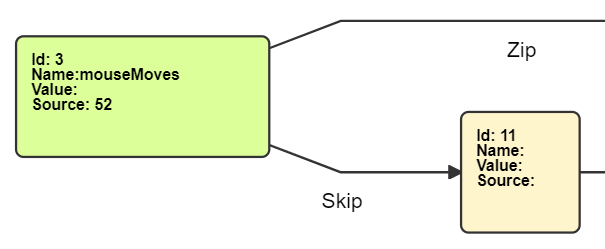
\includegraphics[width=0.4\textwidth]{gfx/NodesCRI2.png}\label{fig:NodesCRI2}}
	\hfill
	\subfloat[CRI version 3.0]{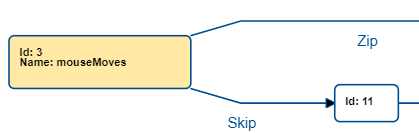
\includegraphics[width=0.4\textwidth]{gfx/NodesCRI3.png}\label{fig:NodesCRI3}}
	\caption{A sample of nodes before and after the changes introduced by this thesis.}
	\label{fig:Nodes}
\end{figure}
%TODO: casing of \emph{Named} node and dependency
Another important aspect to consider is if to display a field on the node directly or in the tooltip. The same principle that applies to general elements of the UI applies here as well. Only values that are necessary to always have present without the need to open every tooltip should be displayed as part of the nodes. We evaluated for each field where it should be located regarding this criteria. The \emph{Name} is important to identify relevant nodes, including those depending or dependent on a \emph{Named} node. The \emph{Id} is required to add Reactive Breakpoints and to identify nodes without a name from one step to another in case the nodes are repositioned due to a new edge being added. The \emph{Value} is normally the property at which developers can see if the JS code of the application works as intended. E.g. an Observable is expected to have a specific value at some point in the execution. The developer can also observe a value passing along the chain of dependencies. For these reasons, the fields \emph{Name}, \emph{Id} and \emph{Value} should be always displayed, as long as they have a value, as part of the node. %TODO: simplify sentence
The \emph{Type} should be hidden in the tooltip, because often what type of Observable the library uses internally does not matter to the developer. E.g. in most scenarios for RxJS, there is no difference between a FromEventObservable and a basic Observable. The information should, however, be still present in the tooltip and not omitted completely because some types of Observables do behave differently than others e.g. RxJS Subject vs Observable. The source code position labeled \emph{Source} is also just used in few special tasks. One example is the user wanting to find the source code corresponding to a node in the graph to modify that code or inspect it further. The \emph{Source} should, therefore, be displayed in the tooltip rather the nodes themselves. The field \emph{Number of Updates} is introduced by this thesis as a way to detect bottlenecks and help identify nodes that cause the generation of a huge amount of steps through excessive value updates in CRI. It is based on the Time Profiling feature of the Reactive Inspector \cite{ReactiveInspector}, but for now, only provides the total number of updates on a node instead of detailed timing and value evaluation information. It is only useful for the purposes mentioned above and, therefore, should not be displayed on the nodes themselves.

An important cognitive task that a user has to do often while using CRI is to track changes between steps in the Dependency Graph History. To track these changes is necessary to understand how the graph is constructed or to track value updates traveling along a chain of dependent Observables. It is, however, not always trivial since the rendering engine \emph{D3.js} \cite{D3JS} used by CRI sometimes moves nodes and edges around to better fit the available space. To help the user with this task, the previous version of CRI already highlighted the nodes that were changed for each step in which a node was changed. We extended this feature to also highlight edges that were updated or added to further decrease the manual searching process. Another feature we added to the UI is a button that hides the tool section of the UI - everything except the menu, History Navigation and Dependency Graph - to allow the user to reduce distractions and free up additional space if they want to focus on the manual examination of the graph and its History. The button is located at the top right corner and has a small arrow icon instead of a text label to reduce its required space in the UI. The option to hide the tool section is especially useful when working with a small screen or a big Dependency Graph. Another button we added to the UI, as part of the menu, was a button to reload the inspected page and, therefore, the Dependency Graph as well. We discovered that reloading was already part of the usual workflow by pressing CTRL F5 and decided to add a button that allows users to achieve this without being aware of the shortcut. An example workflow in which a reload can be used is to create a breakpoint for \emph{dependencyCreated} or \emph{nodeCreated}, and then reloading the application to actually hit the breakpoint.
As figure \ref{fig:Nodes} shows, we also change the colors used in the CRI UI. The node that was changed in the currently viewed step was highlighted by using a red border in the previous version of CRI. The color red is a signal color normally used to show that immediate attention is required or to show that an error has occurred. In traffic signs and lights the color red is used to signal cars to stop or to be aware of dangers. Therefore, we decided to remove it from the normal workflow of CRI. Highlighting the current node is important for the user to immediately identify the change, but it does not require the user's full attention the whole time. It also neither represents an error, therefore the increased cognitive load on the user is unnecessary. The combination of red and green (\emph{Named} nodes) is also problematic for some users with vision deficiency, although as the green is a very bright shaded they should still be able to distinguishable the border on a highlighted \emph{Named} node. Because of these reasons we decided to use blue with light orange as the highlighting that has less contrast between the two shades but still enough to not void the highlighting. To this purpose, we chose a shade of blue and selected the colors for nodes, edges and highlighting from suggestions provided by a color scheme designer \cite{Paletton}. We chose to keep the text color black because it is the most used color for text in general and is easy to read on most colored backgrounds. The nodes that do not correspond to a named variable were left without a background to further reduce the cognitive load. The brain is trained to ignore empty spaces, therefore, making the text and named nodes appear more important.

Another change we introduced to the UI of CRI was the automatic reloading of the Dependency Graph if the Instrumented Files List is changed. This does not reduce the cognitive load on the user but removes the redundant click on the reload button. It is not very useful to change the list of instrumented files without restarting the inspected application and the recording. If the reloading is not done automatically, the user will even be confused that their changes to the Instrumented Files List do not take effect immediately.
	
\section{Connecting abstract graph with JavaScript code}
Nodes in the Dependency Graph that correspond to Observables that are directly assigned to variables provide developers with some form of context. A \emph{Named} node can be used as an anchor to identify the node itself as well as other nodes up and down the chain of dependencies. It helps the user to separate parts of the Dependency Graph that are relevant to the piece of code they want to examine and parts that are currently not relevant. Without any orientation, it is very hard to interpret a shown Dependency Graph. The user can still try to identify nodes by their values or the values of their neighbors, but these values can be missing at certain stages of the application. This all boils down to the issue of connecting the abstract representation of the applications Observables provided by the Dependency Graph with the actual JS source code responsible for those Observables. If an error is detected by examining nodes in the Dependency Graph, the user still has to track down which lines of code are responsible for the issue in order to change them. As mentioned above, \emph{Named} nodes solve this issue in a way, but not all Observables created during runtime are assigned to variables. In fact, even if possible, this is not at all desirable. To the result of each function in a chain of functions to a variable negates most of the benefits of using chained functions in the first place. If the variables are not used by multiple lines of code and are just introduced to support the debugging tool, most of all the disadvantages of \emph{do-debugging} apply as well. We, therefore, evaluated several possibilities to provide nodes that do not have a corresponding variable with additional details that help provide some context to the user. A very basic form of context was already present in the previous versions of CRI in form of the source code position information. This information was, however, not very accurate in case of chained functions because only the start of the source code position information provided by Jalangi was used. In case of chained functions, the source code position actually spans a block that may consist of multiple lines of source code. In addition, information provided did not contain the name of the JS file to which the position belongs. Another downside of this approach is that to look up the source code in another tool apart form CRI and switching back to CRI to check the position of the next node is very cumbersome to execute for more than a few nodes. The developer should be able to easily switch between source code inspection and examining the Dependency Graph because not all issues can be found in either of them when used alone. For example, if there is an issue in an anonymous function, a user cannot find this issue directly in the Dependency Graph. They can only see the result in node values that do not match the values that they expect with the original intention of the code in mind. The main difficulty to achieve this by showing actual source code instead of just the position information is JS code that is used during runtime is instrumented with Jalangi to enable a detailed analysis. Jalangi instrumented code is very hard to read as is shown in listing \ref{lst:Instrumented}.

\begin{lstlisting}[language=JavaScript, caption={Example of RxJS code.},label={lst:Instrumented}]
$sonWallet = J$.W(593, '$sonWallet', J$.F(585, J$.I(typeof $ === 'undefined' ? $ = J$.R(569, '$', undefined, true, true) : $ = J$.R(569, '$', $, true, true)), false)(J$.T(577, '#wallet-son', 21, false)), J$.I(typeof $sonWallet === 'undefined' ? undefined : $sonWallet), true, true);
$fatherWallet = J$.W(625, '$fatherWallet', J$.F(617, J$.I(typeof $ === 'undefined' ? $ = J$.R(601, '$', undefined, true, true) : $ = J$.R(601, '$', $, true, true)), false)(J$.T(609, '#wallet-father', 21, false)), J$.I(typeof $fatherWallet === 'undefined' ? undefined : $fatherWallet), true, true);
\end{lstlisting}

For example, "J\$.W" signals the analysis engine that a write operation is executed when the function is called. This makes it unfeasible to directly show the instrumented code to the user. In addition to being very hard to read, the instrumentation of the source code is an implementation detail of CRI and should not be exposed. Additionally, the code position retrieved from the Jalangi analysis corresponds to the position in the original source code without instrumentation. Note that the JS code that is used during runtime is also dynamically loaded and, therefore, cannot be navigated to out of the box with Chrome DevTools navigation API. Although this is mitigated by adding "//\# sourceURL=" with a custom URL to the bottom of a script. Since this shows the Jalangi instrumented source code that is not useful for a normal user, we decided to tie this to a new option called \emph{CRI Developer Mode} that can be enabled in the options page of CRI. The different approaches discussed in the following section are designed to enable a user to use both the abstract representation and the source code in tandem.
	
\subsection{Evaluated possibilities of displaying source code}
\textbf{Using the \emph{chrome.debugger} API}\\
One possible option is to use the \emph{chrome.debugger} API to open and navigate to the corresponding position of a node. It is easily possible navigating to a line number in a file if the actual file URL, which can differ for dynamically loaded scripts due to many factors, is known. For the reasons explained above, navigating to the instrumented code is not desirable. A non-instrumented version seems to exist in Chrome's \emph{Source} windows as a dynamic script, but it is not actually used at runtime. This approach provides the user with syntax highlighting through Chrome and other features like search with regular expressions. They could also inspect the whole code of the application, not just the piece of code corresponding to a single node if required. The downside of this approach is that the user needs to leave the UI of CRI to access the source information. For a single node, this is not an issue, but it is really cumbersome to inspect the source information of multiple nodes, even if the navigation to the position is automated. It is not possible to highlight the code block that corresponds to the inspected node, which would be especially useful for Observables corresponding to the middle of a block of chained functions. The start and end of the block would have to be manually searched for. Another downside that most likely confuses the user, is that some features of Chrome's DevTools can be used but others will not work and there is no way for CRI to display this disparity. Due to the fact that the code shown to a user is not actually being executed, all features specific to runtime interaction like breakpoints, direct code evaluation or watches will not be usable. A user familiar with Chrome's debugging capabilities will most likely expect them to work properly. A modification of this approach is to display the code in another IDE than Chrome. As some modern IDE's provide a featured to navigate to a function's declaration (in WebStorm called "Go to declaration") which is more scalable than using a String based search for enterprise-sized applications. Although this feature is not available in Chrome, having the user install another IDE and use that in parallel with Chrome will increase the dependencies of CRI and the development effort coupled with that dependency while still suffering from all the downsides of this approach explained above.\\
\textbf{Using an integrated lightweight IDE}\\
Another possibility is to use a file viewer that is opened, for example, as a closable panel to show the full source code. Depending on the implementation this approach can provide full customization of code presentation to the user. In theory, advanced syntax highlighting (syntax highlighting based on the usage and structure of functions like WebStorm does to detect >classes<) could be applied. It is also possible to highlight Observables in the source code while the user hovers over the in the Dependency Graph or even permanently coloring the source code based on the abstract representation. The main problem with this approach is the development effort required to achieve a viable implementation. There is no library available, that we are aware of, that provides the needed functionality and customization options. To develop such a library ourselves requires nearly the same amount of work needed to develop a traditional IDE for JS since it basically is a lightweight JS IDE displayed in a panel of CRI. Another issue with this solution is, in addition to the required development effort, that nodes which are close in the Dependency Graph because they share a dependency do not necessarily correspond to lines of code that are located in close proximity of each other. The code may even be split over several JS files in extreme cases which requires additional view options by any lightweight IDE apart from just showing one JS file.\\ %TODO: search for 'web'
\textbf{Mirroring interactions to a non-instrumented copy of the application}\\
An approach that is possible in theory, but will not withstand a detailed evaluation is to mirror any interaction to the inspected application to another version of it. The idea is to have one application with instrumented JS files, and one where the JS files are not instrumented. This would enable CRI to use another approach like using the \emph{chrome.debugger} API to display the actual source code used at runtime while retrieving analysis data from the instrumented mirror application. It enables the user to use every feature of Chrome or another IDE when debugging JS. The problems introduced by copying the entire application and mirroring any interaction to it, go however, far beyond the doubled resource consumption. %TODO check grammar
 One major issue is the actual recording of user interactions to the original application. There are many tools like Katalon Studio \cite{Katalon} using Selenium \cite{Selenium} that can be used to record and replay interactions to a Web application. These tools are often used to automate the testing of Web applications. Most of these tools are, therefore, designed to ignore certain aspects of interactions like the positioning of elements to make the tests more robust against small changes. Although there are some tools that use pixel positions to record and replay interactions. We could however, find not one tool that records mouse movements and replays them exactly. It is possible to develop a solution oneself, but the mentioned tools solve many issues like always replaying with the exact same screen resolution that is especially important if the layout of the applications UI reacts to different screen resolutions. Another issue with replaying interactions to the copied website are security restrictions imposed by Chrome (and other modern browsers) itself. Chrome restricts some special interactions a user can execute to not be mimicked by a Web application of Chrome extensions to shield users from attackers that use a custom extension or website to influence Web applications outside of their own domain. An example of these restricted interactions is the using of Chrome's Context Menu or the operating system's Clipboard. The reasoning to restrict both are similar and are due to the fact that these features can be used to breach boundaries otherwise monitored by Chrome itself or in case of the Clipboard by the operating system. Since these interactions cannot be mimicked, it is impossible to replay them on the mirror Web application. This voids all other attempts to replay any other interaction because the two applications will desynchronize. The danger of the two applications becoming desynchronized can also be created by Observables or JS code, in general, being time sensitive. For example, an Observable or function that is scheduled to be executed or updated every few milliseconds and has any side effect like increasing a value by one every time the execution happens, needs to match exactly to produce the same result on the mirrored application. This also includes any JS code that is execution order dependent. The same execution order must be maintained, which is especially hard for asynchronous code even though JS's runtime is event-based \cite{EventBasedJS} and does not actually execute code in parallel. In summary, any code dependent on the order of execution or anything timing related has to be mimicked exactly to keep the mirror in sync with the original application, which cannot be guaranteed for all possible applications in a normal environment. \\
\textbf{Source Code Tooltips}
The solution we decided to implement is an extension to the already present tooltips for the nodes. The tooltip for a node that the user hovers over with the mouse pointer changes to a short snippet of source code, corresponding to the node with a few lines of code before and after the relevant code as orientation, that opens if the user presses the CTRL key. For details of the implementations see the next section. This approach, however, has some limitations. If the node belongs to an Observable at the end of a long chain of functions or an anonymous function is used that covers several lines, the code piece may actually be too long to show in a tooltip. If the code is not wrapped properly the code will also be hard to read in a tooltip due to the limited space. In addition, it is also not possible to use any kind of tool inside a tooltip like, for example, searching. As the tooltips are relatively short, this issue is not too serious as the code snippet can quickly be read altogether. Another limitation of this approach is that it is not possible to view the full source code. Since the user cannot change the source code in CRI either, they have to switch to another tool anyway at some point. For now, the Source Code Tooltips do not provide syntax highlighting and, if added in the future, it is important to note that syntax highlighting of short snippets is not very effective in JavaScript. Since JavaScript is dynamically typed language, it is necessary to take usages in other areas of the code into account to correctly highlight language elements beyond reserved keywords. The usefulness of Source Code Tooltips is also greatly decreased if a normal function instead of an anonymous function is passed to an Observable Operator. Some other patterns like using callbacks that are not realized as anonymous functions or functions that create other functions also have the same issue. An example of this is shown in listing \ref{lst:NonLambdaCallback}.

\begin{lstlisting}[language=JavaScript, caption={Example of using a creation function in RxJS.},label={lst:NonLambdaCallback}]
function createFunction(add) {
return (value) => value + add;
}
let fatherWalletValue = sonWalletValue
.map(createFunction(10));
\end{lstlisting}

The source code corresponding to the \emph{Named} node "fatherWalletValue" ranges from line 4 to 5. If the function declaration is not directly placed nearby and, therefore, shown in the tooltip as well, it is not possible to view the implementation of "createFunction" in the UI of CRI.
The greatest benefit of using Source Code Tooltips is that they compliment the Dependency Graph very well. A user does not have to leave CRI to view the corresponding source code and the abstract representation is still the focus of CRI. The tooltips solve the issue of providing additional details for nodes that do not have a corresponding variable name. In fact, they provide additional information for these nodes as well. Using tooltips also has the advantage that they are easy and fast to open and close again. Therefore, the user is able to inspect several tooltips in short sequence. This helps them to find and remember nodes without a corresponding variable name between multiple uses of CRI by other means than remembering the Ids.  The Ids will also change if the user modifies source code that adds new nodes to the Dependency Graph or changes the order of existing ones. Another benefit of using Source Code Tooltips is, that we are able to highlight the exact source code block responsible for a node even within a chain of functions. This is similar to the possibilities when using a  custom lightweight IDE. In contrast to using another full-fledged IDE, however, using tooltips inside CRI does not introduce new dependencies. Another very important feature of using tooltips is that they do not require additional space in the UI. Using a panel that opens on demand as a pop-up or as part of the UI would result in a resize and movement of other UI elements or overlap parts of the UI until it is closed manually. Instead, the normal tooltips open when a user hovers over a node and will be replaced when they hold the CTRL key. If they release the key or move the mouse away from the node, the tooltips will change back or close automatically. This fits well in the already existing workflow of inspecting several nodes with the mouse pointer and is in our opinion very intuitive to use. There was, however, no User Study conducted as part of this thesis to verify that this is true for the majority of users. We chose this approach based on the benefits it provides, even though there are some downsides that will require additional development effort to overcome in the future.
			
\subsection{Implemented Solution - Source Code Tooltips}
In this section, we explain the implementation of the Source Code Tooltips in detail. To retrieve the non-instrumented source code necessary to show in the tooltips, we store them in a dictionary before executing the instrumentation. To provide the correct source code, we first extended the Jalangi library used in this thesis. As explained in chapter \ref{ch:State of the Art}, the used Jalangi library is not actually the full Jalangi framework, but just an in-browser version developed for a single demo. It, therefore, does not support many features of the actual Jalangi. One of these features is the required JS file names that are not included in the position information provided by the demo Jalangi. We, therefore, decided to implement an ad-hoc solution to retrieve the filename. There is no way to determine the source JS file inside the Jalangi analysis because the Jalangi sandbox object is shared by all JS files and the information is not submitted as a parameter to any of the analysis methods. The only solution with minimal changes to the used Jalangi library, which is desirable if it is ever updated, is to replace the J\$ object, with a shallow copy of the original J\$ object. The copy provides the required information and then calls the original. The "W" function of Jalangi is responsible to intercept variable assignments and is used to link nodes to a corresponding variable name. We extended this function and any function responsible for passing the recorded information to the analysis engine to accept the filename as an additional parameter. This replacement is done for every JS file with the corresponding filename. However, since the Jalangi object is quite large, we decided to exclude inline JS scripts directly embedded within the HTML. Inline scripts are often very short and cannot be taken out of their context in the HTML easily. Otherwise, it would be possible to collect every inline script and add them to an external script that is then instrumented and modified with the replacement J\$ object. Therefore, one copy for every inline script is necessary. The shallow copy function of JQuery we used, duplicates only references and not data, but for large objects with many functions, this still has a performance impact if done repeatedly.%TODO check grammar
 But there is actually no downside in omitting the inline scripts from the Jalangi extension, as we simply know that any node with source position information that does not specify a file name to which the position belongs stems from an inline script. The file name of these nodes is labeled as \emph{html}.\\
With the implementation so far, only nodes with a corresponding name will have a Source Code Tooltip, because only variable assignments were reasonable to capture in the previous versions of CRI. We, therefore, extended the analysis engine (located in jalangi-analysis.js) to also intercept function invocations. This enables the recording of source code position information for functions and their parameters. We only check the return value of the intercepted functions if they are an Observable, because the function arguments either are not Observables, or they are created by a call to the Reactive library and should already have been recorded. To retrieve the file name information as well we extended the corresponding functions of the J\$ object similar to the extension of the variable assignment interceptions. With this implementation, it is possible that an Observable is recorded multiple times for the same node, for example, if a node is assigned to a variable inside a function and then returned as the result. In this cases, it is important to always use the position information intercepted from the variable assignment. The reason for this is that if the node in the Dependency Graph has a name from a variable, the Source Code Tooltip should always show the assignment of that variable in order to not confuse the user. Note that since we retrieve the source code position information from the Jalangi analysis, the Source Code Tooltips will not work for nodes that stem from JS files that are not selected for the instrumentation.\\

\begin{figure}[!h]
	\centering
	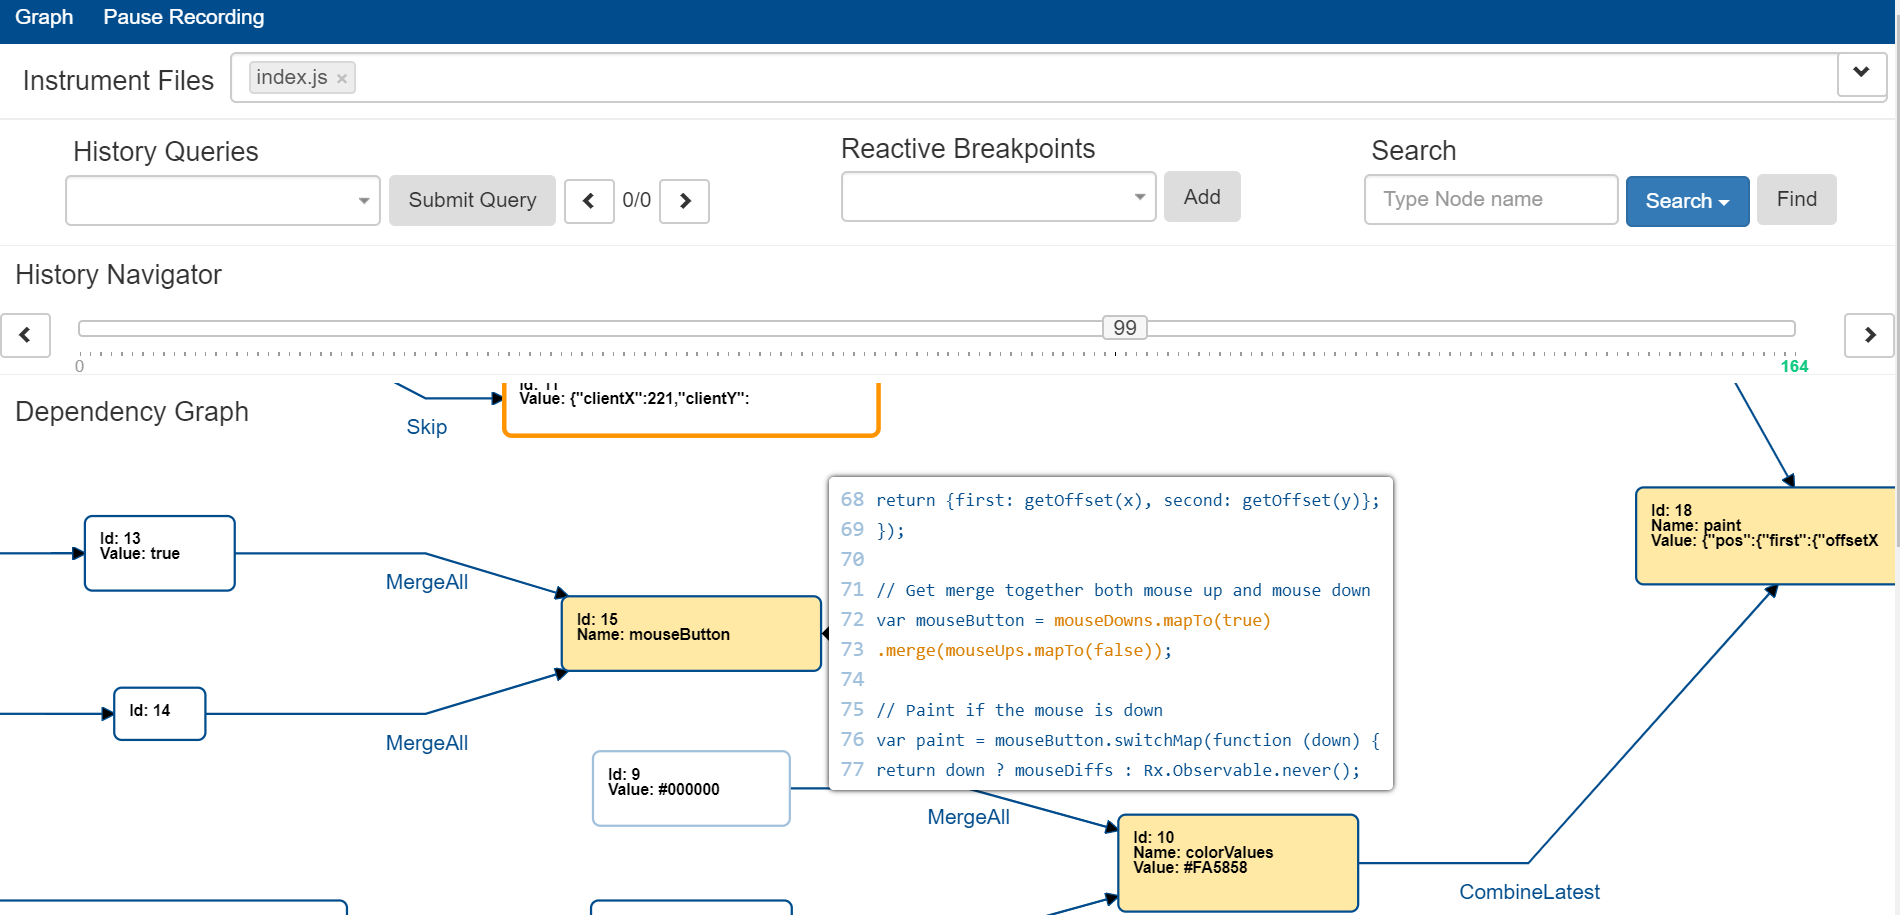
\includegraphics[scale=0.5,trim=0 0 0 0]{gfx/CRI-sampleView.png}
	\caption{A sample of CRI3 UI with opened Source Code Tooltip.}
	\label{fig:CRI}
\end{figure}

We made several additions to the UI of CRI in order to show the Source Code Tooltips in the way described above. The class TooltipManager (located in tooltips.js) handles the creation and displaying of tooltips for all nodes in the Dependency Graph. It adds the UI events used to switch out the tooltips and requests the code needed to construct the Source Code Tooltips from the instrumentation script if the tooltip was not opened before in this step for that specific node. The used tooltip library tipsyJS \cite{Tipsy} that was used in previous versions of CRI is no longer actively developed. We still decided to continue using it, because it provides a simple way to swap out tooltips as it accepts functions for any of the options passed as parameters to the library. However, we had to modify the library to include a fix for a rendering issue that was already submitted as a pull request to the GitHub repository of that library but not accepted due to not being actively developed anymore. To enable the capturing of keyboard events for the Dependency Graph it is necessary to explicitly make the containing HTML element focusable. This is done by adding a \emph{tabindex} attribute. Since the container also needs to have the focus in order to receive the keyboard events, the container is automatically focused when the user moves the mouse pointer over the Dependency Graph. The mouse events used to open or close a Source Code Tooltip of a node are registered when the user hovers over the node and removed when the mouse leaves the area of the node. We also chose to give the user a visual clue if a node has a Source Code Tooltip. This prevents users having to probe each node if a Source Code Tooltip is available. The border of nodes that cannot be linked to a source code position is, therefore, displayed faded. We chose this specific visual representation, because having no Source Code Tooltip means the node does not provide any context information and the normal tooltip will most likely also not provide any valuable information. One could argue that the Location information could now be omitted from the normal tooltips as well, but it is currently the only way for the user to see from which JS file the node originated, since Source Code Tooltips currently do not show the filename. However, this may be changed in the future. An example of the CRI UI with an opened Source Code Tooltip can be seen in figure \ref{fig:CRI}.
	
\section{Rapidly updated Observables}
\label{sec:RapidlyUpdatedObservables}
In this section, we discuss the difficulties when handling applications with rapidly updated Observables and our approach to increasing CRI's ability to cope with them. If the value of one or more Observable is changed rapidly, each change will result in a new step in the Dependency Graph's History. Observables that are, for example, created from timers, mouse movement or a network connection submitting messages change their value very often in a short period of time. The previous version of CRI is not able to handle rapidly updated Observables well. For a detailed performance comparison, see chapter \ref{ch:Evaluation}. However, there were two features added to CRI that enable the user to still use CRI with rapidly updated Observables to some extent. One feature is the option to pause the recording and resume it at a later time. This feature is useful for applications that exceed the limits of CRI slow enough for the user to click the \emph{Pause Recording} button. The user can then examine the recording up to this point without any issues related to performance. This is due to the fact that any user interaction is slow enough for CRI to handle, while steps may be generated by the thousands in the same period of time if the recording is not paused. The other feature that was added is the ability to exclude certain nodes from the recording process, although this is cumbersome to do. The user has to detect and remember the Ids of nodes that are being updated rapidly and then add these Ids to a list located on the options page. This ad-hoc solution can still be useful in certain cases, but in others, the full exclusion of a node will cause errors in the recording process. In the following, we explain the increased demand for resources, the steps implemented to increase performance in this thesis and the limitations of the UI in handling these type of Observables in general. 

\subsection{Difficulties and previous approach}
Not only does the generation of hundreds of steps decrease the expressiveness of each individual step, with some exceptions, but it is also very demanding on computational resources. Messages between Content Scripts, Background Scripts, and the extensions panel have to be transmitted in addition to saving the Dependency Graph's History. This also increases the number of rendering operations of the graph itself which requires a lot of size and position computations. If the computational effort exceeds the capabilities of Chrome and the underlying system, CRI and sometimes even Chrome itself will stop working. There is a threshold regarding the minimum time span between individual updates that if undercut leads to CRI crashing at some point of the execution. The reason for this is the accumulation of requests if more requests are submitted, for example to the Chrome message or storage API, than requests are processed. Over time the resource demand on scheduling requests and managing the JS runtime's event queue increases beyond the available computation power. In this case, the UI becomes unresponsive and Chrome will eventually terminate the extension. In the remainder of this thesis, we will refer to this type of performance issue as \emph{request buildup}.
The steps that are often still significant to a user belong to the start of the History. They usually contain some form of setup phase, were Observables and their Dependencies are created, but there are no values submitted to them yet. An example of this is visible in many of the test applications, as value updates will not occur until the user starts using some form of input element.
%TODO remove can in following sentence
 These steps can still be examined and provide valuable information that is not value-update related about the created Observables. However, the setup phase is not present in each Web application. If the application does not have a setup phase, the History becomes hard to examine. Even if there is a setup phase some parts may be implemented with something like the \emph{Lazy Loading} Pattern \cite{Lazy} in which the creation of Observables will just happen on demand. There may also be no setup at all. It is possible to create Observables dynamically - i.e. the type of dependencies used are a result of some form of computation or configuration - which will not necessarily happen at the start of an application. Another case in which the History becomes hard to examine for a specific task is if the application has multiple busy phases. Such an application may wait for some message from an external component that results in many computations and updated observables. Since the History does not provide an actual timeline and will show steps in a linear sequence these busy phases become very hard to identify and distinguish. 
Another difficulty that stems from the \emph{Pause/Resume Recording} features, is that it results in a broken History. There is no visual feedback in the History Navigation that signals the user a pause has happened. If the recording is paused and later resumed, the steps before and after this gap are not sequential anymore, even though the History indicates the contrary. After the recording was paused, the Dependency Graph will actually show a false image of the variables as their value may differ from the actual variables in the application. This difference only persists until every node is updated once again, but if an Observable or Dependency is created during the pause, it will not be visible at all. The later is somewhat intentional for excessively, dynamically created Observables discussed in section \ref{sec:DynamicallyCreated}. But this still leaves the user to remember at which step they paused the recording or they will get confused if they examine the Dependency Graph while stepping over the gap.
	
\subsection{Reworking the Dependency Graph History}
To reduce the computational resources required to record the Dependency Graph's History and implement a more sophisticated storing mechanism, we reworked the previous implementation. The History records every change to the Dependency Graphs as a new step. While previous versions of CRI stored the whole graph for each step inside an array for simplicity. This means the required memory will increase proportionally with the number of steps. However, the overall memory consumption will not exceed the limits of the environment except in extreme cases, because modern computer systems normally have more than 1GB of RAM available. We decided to use Delta Encoding to reduce the required computations to store succeeding steps. The term Delta Encoding simply describes that instead of storing the full \emph{state} of some entity, for example an object, only the difference to the previous state is stored. This difference is called the Delta and in the case of CRI the \emph{state} is the Dependency Graph in a specific step of the History. The Delta represents the change to the Dependency Graph from one step to the next. This approach is very useful to reduce the size of data that needs to be stored for any stream of data where the Delta between elements in the stream is marginally smaller than an element itself. It is used with great success in video encoding, because the difference between succeeding frames is usually very small, but depending on the resolution of the video, each frame can contain a large amount of information.
As the first step towards implementing Delta Encoding, we modularized the History and introduced \emph{Paging} to it. Although the term \emph{Paging} may be misleading as it usually refers to memory management of the operating system \cite{PagingWiki}, we use it to describe a software engineering pattern as it best describes our approach. This pattern is commonly used to handle large streams of data. What we refer to as \emph{Paging} is the implementation of a (software) Cache structure to the History that loads a subset of succeeding steps. The History will only store a fixed size of steps at once. As soon as the size of this Cache is exceeded, a part of the loaded steps is written to the local disk using the Chrome storage API and removed from the Cache. The Cache is in fact better referred to as a Page, because its content always consists of sequential steps while a software Cache used in programming may contain elements in a random order. If a step is requested that is not currently loaded in the Page, the requested step is loaded along its surrounding steps from the Chrome storage API. The requested step is loaded as the middle of the Page, if possible, to prevent the need to immediately load another step from the local storage, if the user clicks next or previous. This approach keeps the memory consumption of CRI fairly constant and independent of the number of steps in the History, as the maximum number of loaded steps is the size of the Page. We built the Delta Encoding on top of the Paging, to keep the benefits of both approaches.
As mentioned earlier Delta Encoding reduces the data stored to the changes between succeeding steps. These changes are also the relevant information a user of CRI examines when working with the it. Therefore, storing these changes and their types actually provides more useful data and makes the changes easier to query. With the previous approach, the changes between steps needed to be calculated or logged in addition to the History as it was for the History Query feature. For the same reason we implemented Delta Encoding ourselves instead of using a JSON Patch \cite{JSONPatch} based library like the one developed by \emph{Joachim Wester et al.} \cite{JSONPatchImplementation}. The library calculates Deltas itself which consumes additional resources. Delta Encoding also enabled an easy and more robust way to detect the current changed node, and later edge, instead of storing the highlighting in the graph itself. The current change in a step is simply the node or edge affected by the last Delta. With the simplest form of Delta Encoding, a specific step of the History would be created by loading the very first step and then applying all changes stored as Deltas in sequential order on the Dependency Graph stored in that first step. To reduce the computational cost to reconstruct a Dependency Graph for a certain step, an algorithm similar to the one explained at \cite{VideoEncoding} without B-frames was implemented. We call the I-frames \emph{Base Stages}, which store a full graph, and P-frames \emph{Delta Stages}, which only encode the Delta to the previous step. The size of the Delta Window can be configured in code and is currently set to 100, meaning each \emph{Base Stage} will be followed by 100 \emph{Delta Stages} before a new \emph{Base Stage} is created. The implementation is located in history.js. Paging is used to load a subset of continuous \emph{BaseStages} at once and store all other with the Chrome storage API. This is important to cope with the user stepping forward and backwards repeatedly over the threshold between tow \emph{BaseStages}, which would be very resource demanding if only on \emph{Base Stage} would be loaded at once. To increase the Page size also reduces the distinct storage and load commands submitted to the local Chrome storage using the API. The Deltas are used on the graph level and, therefore, always contain the full node or edge that was changed or added, in contrast to a more fine-grained difference. As not all Deltas are easily reversible they always belong to the proceeding \emph{Base Stage} and not to the succeeding \emph{Base Stage}. This is also the reason we did not implement B-frames as used in the original algorithm. To keep the \emph{Delta Stages} that succeed a \emph{Base Stage} linked to it, we store them as part of the \emph{Base Stage} themselves. If a new \emph{Delta Stage} is added or requested that is in the forward direction in regard to the sequential order of the steps, without crossing over any \emph{Base Stage} boundaries, all changes can be directly applied to the current loaded Dependency Graph. If, however, the direction is backwards, the new graph is constructed by emptying the graph, loading the \emph{Base Stage} and then applying all Deltas up to the requested stage. The same logic is used if a random step is requested that is not part of the current Base Stage. This means that loading steps in the forward direction, is always faster than accessing steps at random or backwards. As noted above the forward direction is crucial for the recording process and has a great impact on the performance of CRI when handling applications with rapidly updated Observables. The used algorithm and implementation keep this use case fast and simple. On the other hand, stepping back and random access of steps requires additional computation in comparison to the previous implementation of the History. However, they are only ever triggered by the user themselves which greatly lowers their performance requirements.
The \emph{GraphManager} class handles drawing of the displayed Dependency Graph in the UI and request the loading of a different step from the History when necessary. It also implements the highlighting of the current node or edge. The \emph{History} class handles the actual data, caching and requesting loading of steps from the storage when necessary. It also manages when to switch to the next \emph{Base Stage} instead of adding another \emph{Delta Stage}. The shared, singleton object \emph{stageStorage} provides an Object-Oriented interface, that loads and stores \emph{Base Stages} with their \emph{Delta Stages}, to the key-value based Chrome storage API. \emph{stageStorage} also schedules request internally to ensure that they are handled sequentially and in the correct order. Guaranteeing that stages finish saving before the loading operation is executed. For this reason, the loading operation is asynchronous and uses a callback that is invoked when the loading is done. To achieve the synchronicity of these operations, \emph{stageStorage} uses a queue internally. If an operation finishes storing or loading it will invoke the next operation in the queue.	
	
\subsection{Additional performance improvements}
To further increase the performance of recording new steps in order to enable the usage of CRI with faster updating Observables, we inspected the resource consumption using Memory analysis as well as CPU profiling tools. A comparison of these inspections for this CRI3 and the previous version of CRI is shown in chapter \ref{ch:Evaluation}. We discovered, that for applications with rapidly updated Observables, a huge amount of CPU resources were spent on computations responsible for rendering positions and sizes of the Scalable Vector Graphics (SVG) HTML element used to display the Dependency Graph. A rendering operation was triggered for each newly created step in the History. Throttling these rendering operations and UI updates greatly increased the performance of CRI. Since humans are not able to detect and comprehend changes to the UI happening faster than a certain threshold, decreasing the rendering operations to this threshold will not even be noticed by a user. In fact, we increasing the interval until the next rendering operation is triggered even further. The goal was to use an interval compromising between delay that a user notices and computational resources used to render the graph that often. According to an article by Thomas Burger \cite{Perception} the average human reaction time to visual input is 250ms. Since CRI does not rely on real-time interaction, although the recording process needs to fulfill real-time requirements to a certain degree, they claim that latencies up to 500ms are acceptable before the performance of the user is affected. If a requested result is displayed with a delay of 100ms, the user will experience it as an immediate result. Delays above that will be noticed, but will not annoy most users if they are lower than one second. In order to increase the performance of CRI while not introducing any nuances for the user with applications the extension can easily handle without the throttling, we chose 230ms as a compromise. This is significantly lower than 500ms, but since some Web applications will change node values in intervals smaller than that, we decided to use 230ms as it provided the most fluent experience. In the future it is desirable to add a self regulating mechanism that increases or decreases the delay on demand of the inspected Web application. The lower boundary for the delay should still be 230ms as not to waste computational resources. However, for applications that require extensive resources like the test application \emph{RxJS mario}, there is no fixed upper boundary for the delay. Steps are created so fast that the user is not able to gather any useful information. The displayed Dependency Graph and especially the History will only be useful to examine when the recording is stopped. Therefore, up to that point in time, the UI is unimportant and the delay at which rendering is triggered should be increased accordingly. The upper bound in this scenario is not existing, although it has to be noted, that as explained by Thomas Burger in the article \cite{Perception}, the users performance to perform a task will suffer from the delay until the recording is paused.
There is also the option to exclude some nodes from the recording introduced in CRI1. This is effective if the application only has a few rapidly updated Observables. For most applications with these type of Observables, however, usually many Observables have Dependencies to one or more of the rapidly updated Observables without filtering the submitted values. This leads to chains of rapidly updated Observables that all need to be ignored to drastically reduce the number of generated steps. At this time, CRI does not provide any tools to support the user in ignoring any Observables. Some of the options in this regard are discussed in chapter \ref{ch:Future} and may be the target of further development.

\section{Excessively created Observables}
\label{sec:DynamicallyCreated}
This section discusses the origins of excessively created Observables as well as some of the possible solutions to handle them, however, the implementation of these solutions is outside the scope of this thesis.
In addition to Observables that are rapidly updated, another type of Observable is difficult to handle for CRI and similar tools. If new Observables are created excessively, for example as part of a loop, the Dependency Graph is flooded with new nodes belonging to those Observables. An example where this issue would occur is a Web application that uses networking to connect to a list of clients. The network clients each create an Observable and each message submitted to one of them is gathered in a single Observable that depends on them. If many clients connect or reconnect to the Web application, the Dependency Graph becomes very large and hard to examine. We refer to excessively created Observables as a special type of a Observable for simplicity, although technically the term describes a group of Observables that are created from the same source code. Since these type of Observable usually stem from the same line of source code, the nodes will all share their detailed information like the source position information or name, except for their value. In addition to many long-lasting Observables, the same issue occurs if Observables are created temporarily, for example, as part of a function that performs some type of calculation. Since CRI does not detect if Observables are no longer used, the Dependency Graph shows nodes even after they were deleted by the garbage collector. Another issue for these type of Observables is that if their nodes have a \emph{name}, the current implementation of CRI's History Query and Search feature cannot distinguish them properly because the node identification for some of the queries are based solely on the \emph{name} and does not consider the scope the variable belongs to.
There is no simple way to exclude or handle this type of Observables, as they have numerous sources and behaviors that need different solutions. All possible solutions have in common that they increase the complexity of the recording process.

%TODO: Dependency + Named upper case?
\subsection{Increased recording complexity}
To exclude nodes from the recording of rapidly updated Observables the user is able to specify Ids of the nodes to ignore. However, this approach does not provide a solution for excessively created Observables, since instead of updating existing nodes, new nodes are created. For \emph{Named} nodes the exclusion is possible using the name, but this does not work for any other nodes. For this reason, CRI has to provide rules that specify certain characteristics by which newly created nodes are filtered. In contrast to ignoring the value updates and still creating the nodes, this type of Observables has to be excluded from the recording process completely. Yet, some visual representation of these nodes is required in the Dependency Graph. Detection of nodes that belong to excessively created Observables needs to handle many subcategories of these Observables. One possible solution is to replace the group of nodes with a single pseudo node that merges all nodes of the group. This is not suitable for all categories of excessively created Observables and is only applicable if all outgoing edges have the same target and ingoing edges have the same source. For cases in which these differ, the edges may be displayed with a sophisticated visual graph optimization approach like edge bundling \cite{EdgeBundling}. In this approach, the values of the merged nodes are displayed on the pseudo node. These values cannot be omitted in general even though they differ for every Observable in the group and one group may consist of hundreds of nodes, depending on the inspected Web application. To display these values a scalable UI element is needed that allows the user to inspect any of the values independent of the group size. The detection of nodes to merge into a group is fairly robust when using the source position, although there may be some other cases in which nodes should be merged. As we mentioned earlier there are several possible options to handle these type of Observables, but all have in common that the recording process increases in complexity. If the user should be able to reverse the merging of nodes on demand or a rule-based exclusion is chosen as the approach to handle this issue, the recording becomes customizable. To enable the user to keep the customization over more than one session, it has to be persisted. Since the customization is also highly specific to a single inspected Web application, some form of session or project management. In contrast to the current implementation of excluding nodes via the options page, the loading and storing of this persistent customization should be integrated into the menu of the main UI, because it directly corresponds to the currently displayed Dependency Graph.
	
\section{CRI - A growing project}
At the beginning only one developer, Waqas Abbas was working on the project who was later joined by Pradeep Baradur. They worked independently but parallel for some time and both extended CRI as discussed in section \ref{sec:PreviousCRI}. Their work on CRI was strictly focused on implementing the basic extension itself and then extending it with many features. However, as the project grew and their work later was merged as the first task of this thesis, the focus moved CRI to be a full-fledged project that introduces new maintainability and extensibility requirements. In this section, we describe our approach to increasing development velocity and those requirements by reorganizing the file structure and increasing modularity.

\subsection{Increasing velocity}
In CRI1 the JS files of the extension were mostly organized into directories with files that implement similar or related functionality. For example, all files containing the code corresponding to the recording of nodes from the Reactive libraries were located in the \emph{event-sniffer} directory. As we started working on the project, we discovered that this organization is not suitable at the top level, because it most likely confuses any developer working on the project. The reason for this is the different contexts in which JS files are executed in a Chrome extension. The \emph{window} object representing the global scope of a JS file can be different to the one used in other files. The \emph{window} object in a Content Script is shared among all Content Scripts and provides access to the Document Object Model (DOM) of the inspected Web application. However, the \emph{window} object in JS files that run in the context of the DevTools panel of CRI is specific to that context and provides access to the DOM of CRI's panel. Background Scripts also have their own shared context. In addition, scripts running in these different contexts have access to other subsets of the Chrome API. If the JS files of the extension are organized as in the previous version of CRI, JS files located in the same directory may run in different contexts. To remove this confusion, we separated the JS files at the top level by their context. Background Scripts are located in the \emph{background} directory while Content Scripts are located in the \emph{content-scripts} directory. The scripts that run in the context of the DevTools panel are located in the \emph{devtools} directory. All external libraries are located in the \emph{libraries} directory because some libraries are used in multiple contexts. At any level below the top level separation by context, the scripts are still organized into directories with files sharing similar or related functionality. This reduces the risk for a developer to lose track of the \emph{window} object and access to the Chrome API available for a script.
A large part of documentation for the previous versions of CRI was included in the theses of Waqas Abbas and Pradeep Baradur, however, the number of comments directly providing documentation within the source code were sparse. A developer starting to work on the project had to check the external documentation to comprehend the source code, increasing the time required to do so. Therefore, to further increase development velocity we also added additional source code documentation to reduce the time needed to comprehend the existing code. We measured the number of single- and multi-line comments for both Chrome Reactive Inspector version 2 (CRI2) created by Pradeep Baradur as part of his thesis and the current version of Chrome Reactive Inspector, version 3 (CRI3), to verify that the number increased. The source code of CRI2 contains 231 single- and 32 multi-line comments while the source of CRI3 contains 271 single- and 52 multi-line comments. These numbers include TODO comments, found mostly in CRI3, and commented code, found mostly in CRI2. Only JS files developed in CRI were included in the measurements. 
As the project grew and more and more features were added, some JS files grew above 500 lines of code, for example, \emph{panel.js}. In mind of software engineering aspects like separation of concerns and modularity, long files with multiple independent tasks are not desirable. In addition, the nature of JS as a script language without class definitions (before ECMA6) tempts developers to neglect encapsulation and use many global variables and functions. To increase modularity and encapsulation, which helps to track and correct errors or extend existing code by enclosing the influence of a change or limiting the code that has to be inspected for a specific error, we used the JS closure pattern. A closure prevents variables to be accessed from the outside and makes them effectively private. This works because variables are bound to a function context in JS. In the example seen in listing \ref{lst:closure}, a self-executing function is used to implement the closure pattern that returns a function. It is also possible to use closures to create pseudo-classes in JS that can be instantiated with the \emph{new} keyword. In that case, the self-executing function returns a constructor function that in turn return an object. In addition to both these construct, we used closures to implement singleton objects. An example for this is the \emph{stageStorage.js} file. Using closures prevents the pollution of the global window object (for a specific context) while also documenting that these functions belong together. In addition, they limit the interface to other components of the application to a set of explicitly public variables and functions.
		\begin{lstlisting}[language=JavaScript, caption={Example of RxJS code.},label={lst:closure}]
			var add = (function () {
			var counter = 0;
			return function () {return counter += 1;}
			})();
		\end{lstlisting}
In total, we added nine new classes. The only JS scripts that are still not using a closure to encapsulate their internal logic are the files \emph{background-communication}, \emph{options}, and \emph{panel}. The first two are the only scripts inside their respective context. The \emph{panel} script ties all features together and previously used and provided many globally accessed variables. This increased the development effort to separate individual components and dependencies beyond the scope of this thesis as this was not its main focus. Although several efforts have been made to move some components to their own JS files and to reduce the number of global variables. In the future, the code responsible for the Search and History Query feature is to be extracted too. Ultimately the \emph{panel} should only be responsible to instantiate other classes and delegate events and tasks to them. To further increase modularity and provide developers with a robust and tested pattern for separation of concerns in application with a UI, a common pattern like Model View Controller (MVC) or Model View ViewModel (MVVM) should be used for the CRI DevTools panel.
Code metrics are usually used to verify that modularity and separation of concerns are adhered, while still avoiding high coupling of these modules. However, most code metrics like coupling and cohesion \cite{Coupling} cannot be calculated for a dynamically typed language like JavaScript. Instead of these metrics that provide sound results for Object-Oriented programming, we used more ad-hoc and less robust metrics. In detail, we used the total number of lines, the number of files and the average number of lines per file to provide insight on the extent to which we increased modularity. See the Appendix \ref{ch:Appendix} for the exact results.
	
\subsection{Build process}
CRI provides a packed Chrome extension file that is deployed as the stable version. This packed extension contains by default all files in the chosen subdirectory, including files that are only relevant for developers of CRI like the \emph{.gitignore} file in addition to IDE project files that may even expose sensual information about developers or their development systems. The suggested approach is to implement a custom build process that creates a new directory that only contains files need to run the extension \cite{BuildScript}. We implemented the build process in JS using \emph{NodeJS} \cite{NodeJS} in the \emph{build\_process} project. The reason to use a JS build script in place of any other sophisticated build language is to provide the developers with a familiar language and tools. In the future, this build process may also be used to reduce the size of CRI's JS files by minifying them. 
	\cleardoublepage
	\chapter{Evaluation}
\label{ch:Evaluation}
In this chapter, we evaluate the contributions of this thesis and the general state of the project. On that account, we first examine the changes to the UI, the Source Code Tooltips, and performance improvements. We then verify the most important features of CRI by checking a set of specifications for each test application and discussing the result.

All performance measurements and tests in this chapter were performed with Chrome Version 64.0.3282.140 (Official Build) 64-bit, WebStorm 2017 3.4 and Windows 10 Home 64-bit version 1709 build 16299.192. The used device has 8GB RAM, Intel i7 7500 2.7GHz 4CPUs Processor with integrated Intel(R) HD Graphics 620. Each test application was hosted on the integrated Web server of WebStorm on the local machine. No other applications were running during the execution of the tests, although, background processes and services, as well as, other unpredictable factors have to be taken into account which may have influenced the results of the performance measurements.

\section{Evaluation of Improvements}
This section examines the improvements introduced by this thesis and their implementations. We inspect the changes made to the UI as well as the Source Code Tooltips and their applicability regarding the test applications. At last, we examine the performance improvements introduced by this thesis in comparison with the previous version of CRI.

	\subsection{Changes to the User Interface}
	Most of the changes to the User Interface are, by their nature, hard to evaluate in regards to their usability improvements. The experienced usability of a UI can be highly subjective. The easiest way to achieve consistent evaluation results is, therefore, by collecting and analyzing empirical data, for example through Clickstream analysis \cite{Clickstream}. Since CRI is not yet used in active production systems by a large user base, a User Study would be the usual approach but would exceed the scope of this thesis. However, some changes are still verifiable as improvements. For example, the text per node in the dependency graph was reduced without losing any information. This is clearly a general improvement of usability because the change did not affect any other part of the UI and removed obsolete text. 
	In addition to highlighting a node that was updated in the currently viewed step of the dependency graph history, edge highlighting now provides additional information for the user. This helps track down differences between steps which were not as easily detectable before without affecting other aspects of the UI. Furthermore, there is now an option - the \emph{hide} button - to hide parts of the UI which are not necessary to examine the dependency graph. Although the \emph{hide} button as a new UI element might introduce minor usability issues, it can still be considered an objective improvement - as can the edge highlighting.
	
	%TODO continue

	\subsection{Inspecting Source Code Tooltips}
	The Source Code Tooltips that connect nodes in the dependency graph with the JS code they originate from are created whenever the user hovers over a node and presses the CTRL key. Due to their on-demand nature, their performance impact on the time-critical computations of CRI like the recording process can be neglected. The original JS files are stored in a variable in a content script of CRI that is queried for the lines corresponding to a node if requested. Storing a copy of the whole JS file in addition to the instrumented version, however, should not exceed the memory (i.e. Random Access Memory) of any modern computer that runs Google Chrome. We will examine the robustness of this feature in regards to its accuracy in a later section as part of the test application evaluation. To investigate and verify the usefulness of Source Code Tooltips we examined each test application and calculated the percentage of nodes that gain additional context through this feature. As a \emph{named} node already has some form of context that helps the user to identify it and its dependents, we counted \emph{named} nodes separately. For the exact circumstances and inputs used for each test application see section \ref{sec:EvalTests}. %TODO rephrase Over all? remove paragraph
	 Over all test applications, there were 586 nodes in total. Of these, 440 nodes had a Source Code Tooltip which equals to approximately 75\% of all nodes. Only 199, approximately 33.9\% of all nodes are \emph{named}. This means that the introduction of Source Code Tooltips provided additional means to identify a node to the user for 35.1\% of the total number of nodes. The remaining 146 nodes that cannot yet be linked to specific positions in the source code in part consist of nodes that can be easily interpreted by examining the nodes that depend on them. For example in the test application \emph{RXJS canvas-painting} the node with Id 6 is a \emph{FromEventObservable} created by "Rx.Observable.fromEvent(colorchar,"click")" and is not yet detected by the Jalangi analysis.

	\subsection{Scrutinizing Performance with rapidly updated Observables}
	\label{sec:PerformanceEvaluation}
	In this section, we evaluate the performance improvements resulting from the reworked graph history and the less frequent UI rendering in detail. To this purpose, we developed a new test application for RxJS which is used as a simple benchmark on how well CRI, and in the last part of this section RxFiddle, cope with a simple rapidly updating observable. The application uses an \emph{interval observable} to generate one update every five milliseconds over a period of five seconds. Listing \ref{lst:performanceTestExtract} shows the observable responsible for the updates. The full source code including the termination after five seconds is presented in Appendix \ref{ch:Appendix}.
	
	\begin{lstlisting}[language=JavaScript, caption={Example of RxJS code.},label={lst:performanceTestExtract}]
	var intervalObservable = Rx.Observable.interval(5)
	.timestamp()
	.bufferCount(2, 1)
	.map(function (w) {
	return w[1].timestamp - w[0].timestamp;
	})
	.share();	
	\end{lstlisting}

	To exclude the initial setup of CRI from the gathered performance data we create a \emph{reactive breakpoint} for the \emph{nodeCreated} event of node one ("nodeCreated[1]"), ran the application until it paused at the \emph{reactive breakpoint}, started the performance recording and then continued execution. To record a CPU profile that includes the time spent per function we used the Chrome-JavaScript Profiler. To inspect the memory usage we used the memory tab of Chrome DevTools. The duration of the recordings vary from the actual execution time of the test application in the respective case, because they were started and ended manually. 
	
	\textbf{CPU Profile}
	\begin{figure}[!h]
	\centering
	\subfloat[Chrome Reactive Inspector version 2.0]{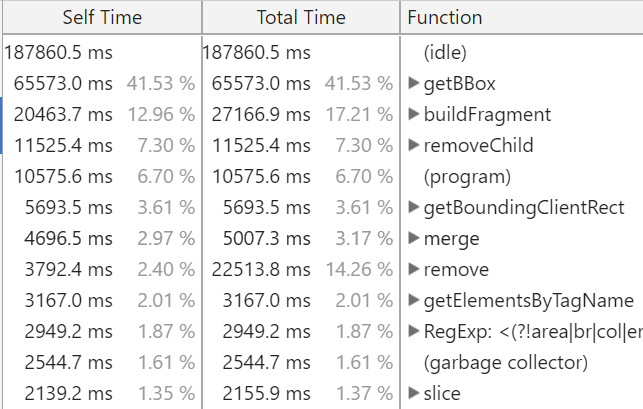
\includegraphics[width=0.49\textwidth]{gfx/CPU_CRI2.png}\label{fig:CPUCRI2}}
	\hfill
	\subfloat[Chrome Reactive Inspector version 3.0]{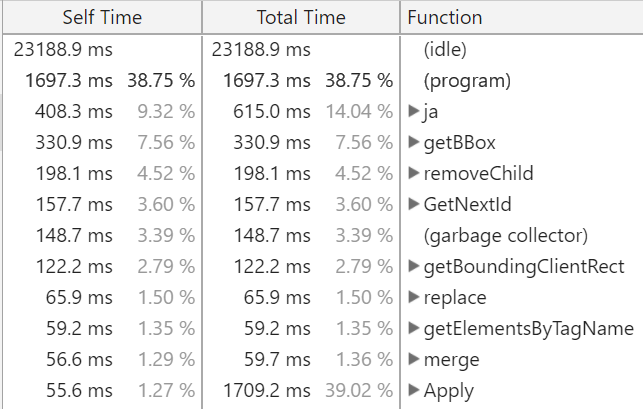
\includegraphics[width=0.49\textwidth]{gfx/CPU_CRI3.png}\label{fig:CPUCRI3}}
	\caption{CPU Profiles recorded by Google Chrome's JavaScript Profiler.}
	\end{figure}
	
	The label "(program)" in the recording entitles native code execution of Chrome. The measured execution time for this label is far less accurate than any other measurement because the individual composition is unclear and can solely increase by stopping the recording at a later point in time due to the limitations of the recording tool.
	
	For CRI2 the execution of PerformanceTest took approximately 154.0 seconds with an overall recording interval of 187.9 seconds. To differentiate between execution time and recording time we selected an area with significantly higher CPU load that should correspond reasonably well to the actual execution time. The largest percentage of \emph{Self Time} (the time spent executing code directly in the function) spent in a single function directly correspond to excessive UI updates - which happen at least once per created step since the slider is updated and triggers the rendering of a new dependency graph for that step. \emph{getBB} (getBoundingBox) calculates the size of nodes in the graph, whereas  \emph{buildFragment}'s impact stems from the \emph{domManip} function of jQuery.
	For CRI3 the execution took approximately 5.5 seconds with an overall recording interval of 23.2 seconds. It is visible that still a sizable amount of time is spent inside UI related computations especially \emph{getBB}. The most time of execution not related to Chromes native code is spent inside the \emph{ja} function of jQuery that cannot easily be tracked down to CRI code. Overall the most time is spent inside Chromes native code, but as described earlier this can have numerous reasons. Due to the nature of changes from CRI2 to CRI3 we are, however, able to account at least part of that execution time to storage operations using the Chrome Storage API. 
	As CRI3 was approximately 28 times faster than CRI2, the performance improvements regarding rapid updates implemented by this thesis were effective. It is, however, worth noting, that CRI2 is barely able to handle this test without crashing - the UI becomes temporarily unresponsive. This probably increases the performance differences between the two versions of CRI more than it is for a test both CRI versions handle well (without the UI becoming temporarily unresponsive). We chose to keep the test as-is to underline the impact of \emph{request buildup} and load exceeding the extension's capacity. 
	As of now CRI3 also has a fixed capacity of updates it is able to handle without crashing, but it is much higher than CRI2's mostly due to the throttling of rendering operations. Basic tools to detect and react to an application exceeding that capacity are already in place for CRI3 and could be easily extended to automatically detect if rendering computations accumulate beyond its limit and increase or decrease the throttle interval for UI updates on demand. Since all steps are recorded even if the rendering is not able to keep up, increasing the throttle time to keep the extension from crashing is a viable approach. The user is then able to pause the recording anytime and examine the steps in details whereas a crash will render CRI useless to the user.
	
	\textbf{Memory Profiling}
	To reveal the impact of a large history on memory consumption we executed the PerformanceTest with a limit of 250ms for both versions of CRI in addition to the execution we used for CPU profiling with a limit of five seconds.
	
	\begin{figure}[!h]
		\centering
		\subfloat[CRI2 - 5s duration]{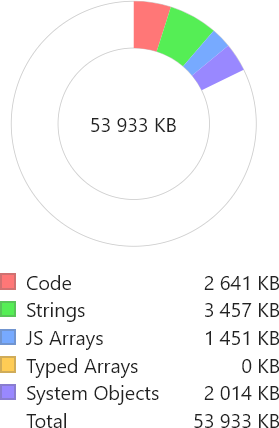
\includegraphics[width=0.3\textwidth]{gfx/RAM_CRI2.png}\label{fig:RAM2}}
		\hspace{1cm}
		\subfloat[CRI3 - 5s duration]{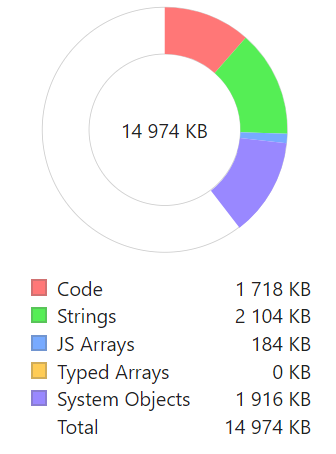
\includegraphics[width=0.3\textwidth]{gfx/RAM_CRI3.png}\label{fig:RAM3}}
		\hspace{10cm} % forces the linebreak between images
		\subfloat[CRI2 - 250ms duration]{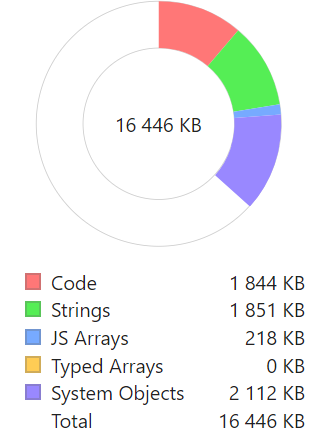
\includegraphics[width=0.3\textwidth]{gfx/RAM_CRI2_250ms.png}\label{fig:RAM2Short}}
		\hspace{1cm}
		\subfloat[CRI3 - 250ms duration]{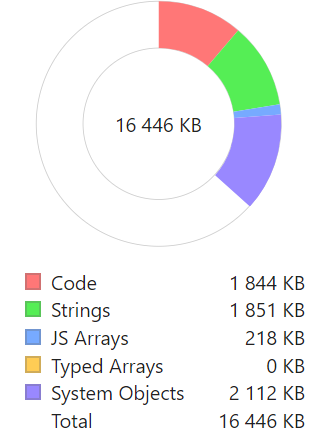
\includegraphics[width=0.3\textwidth]{gfx/RAM_CRI2_250ms.png}\label{fig:RAM3Short}}
		\caption{Memory Profiles recorded and displayed by Google Chrome's Memory DevTool.}
	\end{figure}
	
	For the test execution with the full duration (results visible in figures \ref{fig:RAM2} and \ref{fig:RAM3}) CRI2 used 52.7MB in total while CRI3 used only 14.6MB. The most notable difference in a specific category is the size of the memory used by JS arrays which include the stored dependency graph. In the test with reduced execution time (250ms), CRI2 used approximately 16.1MB of memory while CRI3 used 12.6MB of memory. Both versions of CRI have a similar memory consumption for the test with reduced execution time, although CRI2 shows the dependency graph with a noticeable delay (still less than 5s). Since CRI3's history implements a stream like approach through paging, the memory usage once the size of a single \emph{page} is exceeded is fairly constant and does not increase with the number of steps. As CRI2's history does not support paging the memory usage increases approximately proportional to the number of steps in the history. However, since modern computers have usually more than 1GB of memory, even the higher memory consumption of CRI2 does not have any influence detectable by the user. We made no distinction of CRI3 with Delta Encoding and Paging; and CRI3 just with Paging, because this examination shows that the memory usage is far to low to  imposes any limitation on the overall performance of CRI, even for CRI2.
	
	As there were no significant changes to the recording process of RxJS and BaconJS in CRI, we did not execute separate performance measurements for CRI2 and CRI3 using a test application with BaconJS.
	
	\textbf{Comparison to RxFiddle}\\
	We also examined the performance of RxFiddle with the used test application and compared it to CRI3 to qualify the discussion in section \ref{sec:RxFiddle} on its performance with rapidly updated observables.
	Although RxFiddle does not have performance issues (exceeding a delay of one second when hovering over a node before the tooltip is shown) for approximately one thousand updates on Chrome, if executed with Firefox (57.0.4 (64-bit)) the browser becomes unresponsive for a few seconds. The overall memory consumption of RxFiddle during the test was 52.5MB and the execution took approximately 5.5 seconds - similar to CRI3. As mentioned earlier the memory consumption is not a limiting factor for the overall performance. CRI generates approximately 2700 steps during the test execution while RxFiddle generates approximately one thousand values for each operator in the chain of \emph{intervalObservable} which is displayed in figure \ref{fig:RxFiddlePerformance}. Examining these results any further does not provide additional insight since the tools are based on completely different technologies. RxFiddle uses TypeScript and runs as a Web page while CRI does not use TypeScript, any form of bundling or minifying and runs as a Chrome extension.
	
	\begin{figure}[!h]
		\centering
		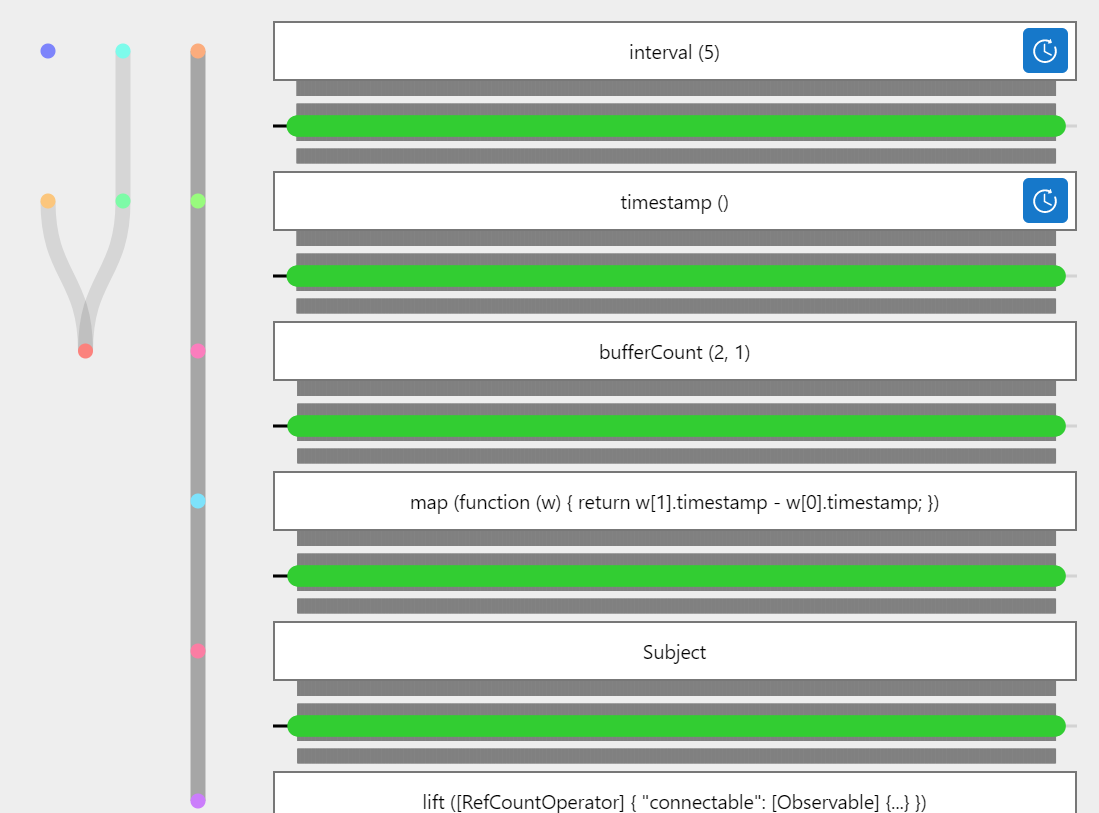
\includegraphics[scale=0.7,trim=0 0 0 0]{gfx/RxFiddleWithTimer.png}
		\caption{Test application PerformanceTest inspected with RxFiddle}
		\label{fig:RxFiddlePerformance}
	\end{figure}
	
\section{Reviewing the Test Applications}
\label{sec:EvalTests}
To establish the current state of the most important features of CRI we compiled a set of specifications that we validated for each of the test applications. They were also designed to provide a baseline for the robustness of the current CRI implementation. Note that we also included specifications targeting features not introduced by this thesis as a means of manual regression testing for the most important aspects of CRI. Since most of these specifications cannot be tested for each node, step and/or case in reasonable time, we specified the exact tests that were performed in order to approximate the results. These test probes should provide a reasonably precise evaluation and, in contrast to some of the specifications, are easy to reproduce in order to verify our results.

\textbf{Specifications}
\begin{itemize}
	\item[Spec1] The dependency graph is shown and all observables that are assigned to a named variable are displayed distinctively. (Test: Up to the first five named observables in the code are all displayed with an orange background.)
	\item[Spec2] The history of the dependency graph can be navigated. It is possible to navigate to the previous, succeeding or a random step in the history. (Test: Jump to the median step; click next five times; click previous five times.)
	\item[Spec3] For each node, no space is occupied by fields that hold no value in neither the node itself nor its tooltip.
	\item[Spec4] The ids of the nodes start at one and are continuous. If the test application is started again with the exact same inputs, each node has the same id as in the last execution.
	\item[Spec5] The Source Code Tooltips show and highlight the corresponding lines of code for each node that has one. (Test: If possible, choose two nodes, one that corresponds to the middle of a chain of reactive function calls and one that corresponds to the end of a chain of reactive function calls. For both nodes check if the highlighting is correct.)
	\item[Spec6] The node or edge that was updated in a step is highlighted. (Test: Check this behavior for the first ten steps in the history.)
	\item[Spec7] The history queries can be used to search for a specific event in the history. (Test: Queries for \emph{evaluationYielded} and \emph{nodeUpdated} find the corresponding steps for the first named node.)
	\item[Spec8] The graph can be searched, the matching node(s) is/are highlighted and if the search is reset the original coloring is restored. (Test: Search for the dependencies and dependents of the first named node and then reset the search.)
	\item[Spec9] \emph{Reactive breakpoints} can be used to pause the debugger when a specific event occurs. (Test: \emph{a)} A breakpoint set for the first node created will break at step one. \emph{b)} A breakpoint for the first node updated will break before the value is updated in the original observable. Note: The value will be already updated in the CRI UI.)
\end{itemize}

We excluded some of the test applications that were used in the prior works targeting CRI from this evaluation because they no longer work due to outside influences or did not provide any additional value. The results of this evaluation are visible in tables \ref{tab:RxJSa}, \ref{tab:RxJSb} and \ref{tab:BaconJS}. For the following statistics, we interpreted \emph{ambiguity} between nodes with the same name, labeled with \emph{Am}, as if the check failed because CRI is not able to handle them properly yet. \emph{N.A.} means that the check was not applicable e.g. because there were no \emph{named} nodes in the dependency graph and the check is dependent on \emph{named} nodes. We, therefore, treated \emph{N.A.} as a success. Due to specification number 9 having two parts that can fail or succeed individually we treated their result separately in the following statistic. Overall 388 of 420 single checks (10 per test application) were successful. The specifications number 2 up to number 6 in addition to number 9 \emph{b)} verified for all test applications. The 32 checks that failed fall into four categories. All checks labeled with \emph{ambiguity} are the result of CRI not being able to handle multiple nodes with the same name. This happens for example if a named variable is created inside a loop. The history query and search feature will not be able to correctly distinguish between the ambiguous nodes and any operation that requires a name will only find the node added last to the dependency graph and show the result solely for that node. Specification 9 \emph{a)} failed for all RxJS applications where the node with Id 1 is not added by the Jalangi analysis. It seems the RxJS interception records nodes out of order in certain circumstances. We verified that this behavior already existed in the previous versions of CRI2 by executing the same check with \emph{RxJS son-father-wallet} application. The failed checks for specification number 8 denote fails to identify every dependent or dependency. This seems to correspond to observables being dynamically created but it will not fail for every dynamically created observable. In case of the check for the \emph{RxJS crop} application, this behavior is not consistent with previous versions of CRI and stems from changes in CRI3, however, the issue in the \emph{RxJS stopwatch} application was already present in CRI2.
In the newly added test application \emph{RxJS InlineScriptTest}, that was added to verify CRI working with JS code directly embedded within HTML, CRI does not detect every \emph{named} observable, because the extension is currently not able to detect and intercept JS code inside HTML attributes.
The failed check for specification number 1 in the \emph{BaconJS blog\_url} application is the result of BaconJS interception not being able to detect the used observables correctly. The \emph{named} observable is not detected and in addition, each change to the used observable in the JS code creates a new node in the dependency graph. This has to be counted as a complete breakdown of the recording for this test application and is consistent with previous versions of CRI. The remaining failed check for specification number 1 in the \emph{RxJS alphabetinvasion} application also denotes a full breakdown of the recording. It seems the current implementation is not able to detect the observables correctly or, in most cases, at all. This behavior is also consistent with previous versions of CRI and is the result of the patterns used in this application. The observables that were not recorded correctly are never assigned and no reactive operator is used on them except of \emph{subscribe} or \emph{unsubscribe}. An example of this is visible in listing \ref{lst:AlphabetInvasionExtract}.

\begin{lstlisting}[language=JavaScript, caption={Extract of RxJS AlphabetInvasion test application.},label={lst:AlphabetInvasionExtract}]
Rx.Observable.timer(750).subscribe(function () {
self.playfield.removeChild(enemy);
});	
\end{lstlisting}

For the test application \emph{RxJS mario} we added a \emph{reactive breakpoint} on the last dependency that is created because the excessive use of timers and rapidly updating observables still causes CRI to crash after a few seconds. This is probably the result of \emph{request buildup} due to a large number of calls to the communication API of Chrome, but it is hard to provide a sufficient proof because Chrome itself will stop responding as well.

\begin{table}[]
	\centering
	\resizebox{\textwidth}{!}{%
	\begin{tabular}{lllllllllllll}
		alphabetinvasion & mario & PerformanceTest & animated-image & animationtest & backpressure & crop & creaditcard-drag & draw-with-combine-latest & earthquake & simple-databinding & stopwatch &   \\
		Spec 1           & \mno     & \myes               & \myes              & \myes             & \myes            & \myes    & \myes                & \myes                        & \myes          & \myes                  & \myes         & \myes \\
		Spec 2           & \myes     & \myes               & \myes              & \myes             & \myes            & \myes    & \myes                & \myes                        & \myes          & \myes                  & \myes         & \myes \\
		Spec 3           & \myes     & \myes               & \myes              & \myes             & \myes            & \myes    & \myes                & \myes                        & \myes          & \myes                  & \myes         & \myes \\
		Spec 4           & \myes     & \myes               & \myes              & \myes             & \myes            & \myes    & \myes                & \myes                        & \myes          & \myes                  & \myes         & \myes \\
		Spec 5           & \myes     & \myes               & \myes              & \myes             & \myes            & \myes    & \myes                & \myes                        & \myes          & \myes                  & \myes\footnote[2]      & \myes \\
		Spec 6           & \myes     & \myes               & \myes              & \myes             & \myes            & \myes    & \myes                & \myes                        & \myes          & \myes                  & \myes         & \myes \\
		Spec 7           & N.A   & \myes               & \myes              & \myes             & \myes            & \myes    & \myes                & \myes                        & \myes          & N.A., \myes             & \myes         & \myes \\
		Spec 8           & N.A.  & \myes               & \myes              & \myes             & \myes            & \myes    & \mno                & \mno                        & \myes          & \myes                  & \myes         & \mno \\
		Spec 9           & \mno\footnote[3],\myes   & \mno\footnote[3],\myes             & \mno\footnote[3],\myes            & \mno\footnote[3],\myes           & \mno\footnote[3],\myes          & \mno\footnote[3],\myes  & \mno\footnote[3],\myes              & \myes                        & \mno\footnote[3],\myes\footnote[1]    & \mno\footnote[3],\myes               & \myes         & \myes
	\end{tabular}%
}
\caption{RxJS test applications a)}
\label{tab:RxJSa}
\end{table}

\begin{table}[]
	\centering
	\resizebox{\textwidth}{!}{%
	\begin{tabular}{lllllllllllllll}
		subjects-examples & wiki-updates & smart-counter & state-store & letter-counter & son-father-wallet & movie-search & follow-the-mouse & drag-and-drop & canvas-painting & twitter-follow-box & rest-api-call & image-sampler & InlineScriptTest &     \\
		Spec 1            & \myes            & \myes             & \myes           & \myes              & \myes                 & \myes            & \myes                & \myes             & \myes               & \myes                  & \myes             & \myes             & \myes                & \mno   \\
		Spec 2            & \myes            & \myes             & \myes           & \myes              & \myes                 & \myes            & \myes                & \myes             & \myes               & \myes                  & \myes             & \myes             & \myes                & \myes   \\
		Spec 3            & \myes            & \myes             & \myes           & \myes              & \myes                 & \myes            & \myes                & \myes             & \myes               & \myes                  & \myes             & \myes             & \myes                & \myes   \\
		Spec 4            & \myes            & \myes             & \myes           & \myes              & \myes                 & \myes            & \myes                & \myes             & \myes               & \myes                  & \myes             & \myes             & \myes                & \myes   \\
		Spec 5            & \myes\footnote[2]         & \myes             & \myes           & \myes              & \myes                 & \myes            & \myes                & \myes             & \myes               & \myes                  & \myes             & \myes             & \myes                & \myes   \\
		Spec 6            & \myes            & \myes             & \myes           & \myes              & \myes                 & \myes            & \myes                & \myes             & \myes               & \myes                  & \myes             & \myes             & \myes                & \myes   \\
		Spec 7            & \myes            & \myes             & \myes           & \myes              & \myes                 & \myes            & \myes                & \myes             & \myes               & \myes                  & \myes             & \myes             & \myes                & \myes   \\
		Spec 8            & \myes            & \myes             & \mno           & \myes              & \myes                 & \myes            & \myes                & \myes             & \mno               & \myes                  & \myes             & \myes             & \myes                & \mno   \\
		Spec 9            & \myes            & \myes             & \mno\footnote[3],\myes         & \mno\footnote[3],\myes            & \mno\footnote[3],\myes               & \mno\footnote[3],\myes          & \myes                & \myes             & \myes               & \mno\footnote[3],\myes                & \myes             & \mno\footnote[3],\myes           & \mno\footnote[3],\myes              & \mno\footnote[3],\myes
	\end{tabular}%
}
\caption{RxJS test applications b)}
\label{tab:RxJSb}
\end{table}

\begin{table}[]
	\centering
	\resizebox{\textwidth}{!}{%
	\begin{tabular}{llllllllllllllllll}
		timer  & blog\_url & comb-lock & dragdrop & events & operators & son-father-wallet split file test & operators-and-events & son-father-wallet & up-down-counter & form-validation & movie-search & bar-chart & websocket-wikipedia & multiselect-card & true-false-logger & drawing &   \\
		Spec 1 & \myes         & \mno         & \myes        & \myes      & N.A.       & \myes                                 & \myes                    & \myes                 & \myes               & \myes               & \myes            & \myes         & \myes                   & \myes                & \myes                 & \myes       & \myes \\
		Spec 2 & \myes         & \myes         & \myes        & \myes      & \myes         & \myes                                 & \myes                    & \myes                 & \myes               & \myes               & \myes            & \myes         & \myes                   & \myes                & \myes                 & \myes       & \myes \\
		Spec 3 & \myes         & \myes         & \myes        & \myes      & \myes         & \myes                                 & \myes                    & \myes                 & \myes               & \myes               & \myes            & \myes         & \myes                   & \myes                & \myes                 & \myes       & \myes \\
		Spec 4 & \myes         & \myes         & \myes        & \myes      & \myes         & \myes                                 & \myes                    & \myes                 & \myes               & \myes               & \myes            & \myes         & \myes                   & \myes                & \myes                 & \myes       & \myes \\
		Spec 5 & \myes         & \myes         & \myes        & \myes      & \myes\footnote[2]     & \myes                                 & \myes                    & \myes                 & \myes               & \myes               & \myes            & \myes         & \myes                   & \myes                & \myes                 & \myes       & \myes \\
		Spec 6 & \myes         & \myes         & \myes        & \myes      & \myes         & \myes                                 & \myes                    & \myes                 & \myes               & \myes               & \myes            & \myes         & \myes                   & \myes                & \myes                 & \myes       & \myes \\
		Spec 7 & \myes         & N.A.       & Am       & N.A.,\myes & N.A.       & \myes                                 & Am                   & \myes                 & \myes               & \myes               & \myes            & \myes         & \myes                   & \myes                & \myes                 & \myes       & \myes \\
		Spec 8 & \myes         & N.A.       & Am       & \myes      & N.A.       & \mno                                 & Am                   & \myes                 & \myes               & \myes               & \myes            & \mno         & \myes                   & \myes                & \myes                 & \myes       & \myes \\
		Spec 9 & \myes         & \myes         & \myes        & \myes      & \myes         & \myes                                 & \myes                    & \myes                 & \myes               & \myes               & \myes            & \myes         & \myes                   & \myes                & \myes                 & \myes       & \myes
	\end{tabular}%
}
\caption{BaconJS test applications}
\label{tab:BaconJS}
\end{table}
\footnotetext[1]{The node with Id 2 was used because the node with Id 1 is never updated}
\footnotetext[2]{The middle of a reactive function chain could not be examined because no function chain was long enough.}
\footnotetext[3]{The breakpoint pauses program execution at the right step, but since nodes are added out of order the node with Id 2 is already added to the dependency graph}

\subsection{Summary}
We examined the set of specifications for each of the test applications and found several issues. The problems with ambiguous variable names and out-of-order recording of nodes, issues that should be resolved at some point, do not break the overall usefulness of CRI. This is because the dependency graph can still be examined and other features work as well, even if they are not directly affected. In contrast, the issues with recording in the test applications \emph{RxJS alphabetinvasion} and \emph{BaconJS blog\_url} cause the extension to display an incomplete dependency graph. This greatly reduces the usefulness of the CRI with these applications.
All issues found should be the target of further development to increase the robustness of CRI, but issues in recording observables should clearly be prioritized.
	\cleardoublepage
	% contribution and future


% Minimize js and css during release build

% extending tools to work with the graph for big applications
	% magnifying glass
	% multi js file support needs improvements - 

% Solution management

% marking the setps where the recording was paused - because if the recording is continued the gap may lead to 
% wrong assumptions about the changes

% IDE extension like eclipse or webstorm that uses the extension to record data and control the debugger.
 % would enable multi window and toolbar support
 % syntax highlighting (snippets would be directly linkable)
 % would enable use of already existing IDE features
 % con: narrows usability and target users, because it would be no longer portable(depending on IDE)
 	% would have more dependencies and would have to cope with additional required changes due to changes in the IDE after
 	% an update
 	
% ecma6 import support and bundled Rx/Bacon detection, + typescript
	% currently searches for <script Rx.js/Bacon.js>
	% if all used libraries are bundled and only own project files are not
	% will not work
	% all module/file loaders are not supported yet e.g. require.js since module loading prior to ecma6 is a diverse field
	% and most applications use one this is one of the main obstacles before the extension can be used by a wider audience (see temp_references)
	% ecma6 import references file not necessarily in html as <script>
	%TODO check if above is true
	%TODO check if typescript compilatino to un-bundled js is possible
	%possible solution: since scripts are side loaded, append a detection function to the bottom of each loaded javascript file that sends
	% a message to the extension if the "Bacon" or "Rx" object is present.
	\cleardoublepage
http://requirejs.org/

Top in JavaScript Libraries and Functions · Week beginning Jan 01nd 2018
Place 14 (from 03.01.2018)
https://trends.builtwith.com/javascript/RequireJS
	
	\listoffigures
	\lstlistoflistings
%	\listoftables
	
%	\nocite{*}
	\printbibliography
	
	\begin{appendices}
		\chapter{APPENDIX}
\label{ch:Appendix}
\section{Ad-hoc code metrics for CRI2 and CRI3}
The lines of code include comments, lines containing only brackets and empty lines.
CRI2 has 8 own JS files with 2353 total and 294 average lines of code per file. The scripts \emph{background}, \emph{devtools} and \emph{content-script-end} are empty and were ignored for these measurements.
CRI3 has 19 own JS files with 3580 total and 188 average lines of code per file.
	\end{appendices}

	
\end{document}